\documentclass[a4paper, 12pt]{book}
%\documentclass[a4paper, 12pt, draft]{book}  Nalogo preverite tudi z opcijo draft, ki vam bo pokazala, katere vrstice so predolge!



\usepackage[utf8x]{inputenc}   % omogoča uporabo slovenskih črk kodiranih v formatu UTF-8
\usepackage[slovene,english]{babel}    % naloži, med drugim, slovenske delilne vzorce
\usepackage[pdftex]{graphicx}  % omogoča vlaganje slik različnih formatov
\usepackage{fancyhdr}          % poskrbi, na primer, za glave strani
\usepackage{amssymb}           % dodatni simboli
\usepackage{amsmath}           % eqref, npr.
%\usepackage{hyperxmp}
\usepackage[hyphens]{url}  % dodal Solina
\usepackage{comment}       % dodal Solina

\usepackage[pdftex, colorlinks=true,
						citecolor=black, filecolor=black, 
						linkcolor=black, urlcolor=black,
						pagebackref=false, 
						pdfproducer={LaTeX}, pdfcreator={LaTeX}, hidelinks]{hyperref}

\usepackage{color}       % dodal Solina
\usepackage{soul}       % dodal Solina

\usepackage{listings}
\lstset{basicstyle=\ttfamily}
\renewcommand{\lstlistingname}{Izsek izvorne kode}% Listing -> Algorithm
\renewcommand{\lstlistlistingname}{Seznam izsekov izvorne kode}% List of Listings -> List of Algorithms

%%%%%%%%%%%%%%%%%%%%%%%%%%%%%%%%%%%%%%%%
%	DIPLOMA INFO
%%%%%%%%%%%%%%%%%%%%%%%%%%%%%%%%%%%%%%%%
\newcommand{\ttitle}{Zasnova in razvoj platforme za spremljanje metrik HTML5 spletnih aplikacij}
\newcommand{\ttitleEn}{Design and implementation of platform for monitoring metrics of HTML5 web applications}
\newcommand{\tsubject}{\ttitle}
\newcommand{\tsubjectEn}{\ttitleEn}
\newcommand{\tauthor}{Miha Jamšek}
\newcommand{\tkeywords}{metrike, html, html5, splet, spletne aplikacije, spa, platforma, rum, spremljanje, čas nalaganja}
\newcommand{\tkeywordsEn}{metrics, html, html5, web, web applications, spa, platform, rum, monitoring, load time}


%%%%%%%%%%%%%%%%%%%%%%%%%%%%%%%%%%%%%%%%
%	HYPERREF SETUP
%%%%%%%%%%%%%%%%%%%%%%%%%%%%%%%%%%%%%%%%
\hypersetup{pdftitle={\ttitle}}
\hypersetup{pdfsubject=\ttitleEn}
\hypersetup{pdfauthor={\tauthor, mj6243@student.uni-lj.si}}
\hypersetup{pdfkeywords=\tkeywordsEn}


 


%%%%%%%%%%%%%%%%%%%%%%%%%%%%%%%%%%%%%%%%
% postavitev strani
%%%%%%%%%%%%%%%%%%%%%%%%%%%%%%%%%%%%%%%%  

\addtolength{\marginparwidth}{-20pt} % robovi za tisk
\addtolength{\oddsidemargin}{40pt}
\addtolength{\evensidemargin}{-40pt}

\renewcommand{\baselinestretch}{1.3} % ustrezen razmik med vrsticami
\setlength{\headheight}{15pt}        % potreben prostor na vrhu
\renewcommand{\chaptermark}[1]%
{\markboth{\MakeUppercase{\thechapter.\ #1}}{}} \renewcommand{\sectionmark}[1]%
{\markright{\MakeUppercase{\thesection.\ #1}}} \renewcommand{\headrulewidth}{0.5pt} \renewcommand{\footrulewidth}{0pt}
\fancyhf{}
\fancyhead[LE,RO]{\sl \thepage} 
%\fancyhead[LO]{\sl \rightmark} \fancyhead[RE]{\sl \leftmark}
\fancyhead[RE]{\sc \tauthor}              % dodal Solina
\fancyhead[LO]{\sc Diplomska naloga}     % dodal Solina


\newcommand{\BibTeX}{{\sc Bib}\TeX}

%%%%%%%%%%%%%%%%%%%%%%%%%%%%%%%%%%%%%%%%
% naslovi
%%%%%%%%%%%%%%%%%%%%%%%%%%%%%%%%%%%%%%%%  


\newcommand{\autfont}{\Large}
\newcommand{\titfont}{\LARGE\bf}
\newcommand{\clearemptydoublepage}{\newpage{\pagestyle{empty}\cleardoublepage}}
\setcounter{tocdepth}{1}	      % globina kazala

%%%%%%%%%%%%%%%%%%%%%%%%%%%%%%%%%%%%%%%%
% konstrukti
%%%%%%%%%%%%%%%%%%%%%%%%%%%%%%%%%%%%%%%%  
\newtheorem{izrek}{Izrek}[chapter]
\newtheorem{trditev}{Trditev}[izrek]
\newenvironment{dokaz}{\emph{Dokaz.}\ }{\hspace{\fill}{$\Box$}}

%%%%%%%%%%%%%%%%%%%%%%%%%%%%%%%%%%%%%%%%%%%%%%%%%%%%%%%%%%%%%%%%%%%%%%%%%%%%%%%
%% PDF-A
%%%%%%%%%%%%%%%%%%%%%%%%%%%%%%%%%%%%%%%%%%%%%%%%%%%%%%%%%%%%%%%%%%%%%%%%%%%%%%%


%%%%%%%%%%%%%%%%%%%%%%%%%%%%%%%%%%%%%%%% 
% define medatata
%%%%%%%%%%%%%%%%%%%%%%%%%%%%%%%%%%%%%%%% 
\def\Title{\ttitle}
\def\Author{\tauthor, mj6243@student.uni-lj.si}
\def\Subject{\ttitleEn}
\def\Keywords{\tkeywordsEn}

%%%%%%%%%%%%%%%%%%%%%%%%%%%%%%%%%%%%%%%% 
% \convertDate converts D:20080419103507+02'00' to 2008-04-19T10:35:07+02:00
%%%%%%%%%%%%%%%%%%%%%%%%%%%%%%%%%%%%%%%% 
\def\convertDate{%
    \getYear
}

{\catcode`\D=12
 \gdef\getYear D:#1#2#3#4{\edef\xYear{#1#2#3#4}\getMonth}
}
\def\getMonth#1#2{\edef\xMonth{#1#2}\getDay}
\def\getDay#1#2{\edef\xDay{#1#2}\getHour}
\def\getHour#1#2{\edef\xHour{#1#2}\getMin}
\def\getMin#1#2{\edef\xMin{#1#2}\getSec}
\def\getSec#1#2{\edef\xSec{#1#2}\getTZh}
\def\getTZh +#1#2{\edef\xTZh{#1#2}\getTZm}
\def\getTZm '#1#2'{%
    \edef\xTZm{#1#2}%
    \edef\convDate{\xYear-\xMonth-\xDay T\xHour:\xMin:\xSec+\xTZh:\xTZm}%
}

\expandafter\convertDate\pdfcreationdate 

%%%%%%%%%%%%%%%%%%%%%%%%%%%%%%%%%%%%%%%%
% get pdftex version string
%%%%%%%%%%%%%%%%%%%%%%%%%%%%%%%%%%%%%%%% 
\newcount\countA
\countA=\pdftexversion
\advance \countA by -100
\def\pdftexVersionStr{pdfTeX-1.\the\countA.\pdftexrevision}


%%%%%%%%%%%%%%%%%%%%%%%%%%%%%%%%%%%%%%%%
% XMP data
%%%%%%%%%%%%%%%%%%%%%%%%%%%%%%%%%%%%%%%%  
\usepackage{xmpincl}
\includexmp{pdfa-1b}

%%%%%%%%%%%%%%%%%%%%%%%%%%%%%%%%%%%%%%%%
% pdfInfo
%%%%%%%%%%%%%%%%%%%%%%%%%%%%%%%%%%%%%%%%  
\pdfinfo{%
    /Title    (\ttitle)
    /Author   (\tauthor, mj6243@student.uni-lj.si)
    /Subject  (\ttitleEn)
    /Keywords (\tkeywordsEn)
    /ModDate  (\pdfcreationdate)
    /Trapped  /False
}


%%%%%%%%%%%%%%%%%%%%%%%%%%%%%%%%%%%%%%%%%%%%%%%%%%%%%%%%%%%%%%%%%%%%%%%%%%%%%%%
%%%%%%%%%%%%%%%%%%%%%%%%%%%%%%%%%%%%%%%%%%%%%%%%%%%%%%%%%%%%%%%%%%%%%%%%%%%%%%%

\begin{document}
\selectlanguage{slovene}
\frontmatter
\setcounter{page}{1} %
\renewcommand{\thepage}{}       % preprecimo težave s številkami strani v kazalu
\newcommand{\sn}[1]{"`#1"'}                    % dodal Solina (slovenski narekovaji)

%%%%%%%%%%%%%%%%%%%%%%%%%%%%%%%%%%%%%%%%
%naslovnica
 \thispagestyle{empty}%
   \begin{center}
    {\large\sc Univerza v Ljubljani\\%
      Fakulteta za računalništvo in informatiko}%
    \vskip 10em%
    {\autfont \tauthor\par}%
    {\titfont \ttitle \par}%
    {\vskip 3em \textsc{DIPLOMSKO DELO\\[5mm]         % dodal Solina za ostale študijske programe
%    VISOKOŠOLSKI STROKOVNI ŠTUDIJSKI PROGRAM\\ PRVE STOPNJE\\ RAČUNALNIŠTVO IN INFORMATIKA}\par}%
    UNIVERZITETNI  ŠTUDIJSKI PROGRAM\\ PRVE STOPNJE\\ RAČUNALNIŠTVO IN INFORMATIKA}\par}%
%    INTERDISCIPLINARNI UNIVERZITETNI\\ ŠTUDIJSKI PROGRAM PRVE STOPNJE\\ RAČUNALNIŠTVO IN MATEMATIKA}\par}%
%    INTERDISCIPLINARNI UNIVERZITETNI\\ ŠTUDIJSKI PROGRAM PRVE STOPNJE\\ UPRAVNA INFORMATIKA}\par}%
%    INTERDISCIPLINARNI UNIVERZITETNI\\ ŠTUDIJSKI PROGRAM PRVE STOPNJE\\ MULTIMEDIJA}\par}%
    \vfill\null%
    {\large \textsc{Mentor}: prof. dr. Matjaž B. Jurič\par}%
    {\vskip 2em \large Ljubljana, 2019 \par}%
\end{center}
% prazna stran
%\clearemptydoublepage      % dodal Solina (izjava o licencah itd. se izpiše na hrbtni strani naslovnice)

%%%%%%%%%%%%%%%%%%%%%%%%%%%%%%%%%%%%%%%%
%copyright stran
\thispagestyle{empty}
\vspace*{8cm}

\noindent
{\sc Copyright}. 
Rezultati diplomske naloge so intelektualna lastnina avtorja in Fakultete za računalništvo in informatiko Univerze v Ljubljani.
Za objavo in koriščenje rezultatov diplomske naloge je potrebno pisno privoljenje avtorja, Fakultete za računalništvo in informatiko ter mentorja.
Izvorna koda diplomskega dela, njeni rezultati in v ta namen razvita programska oprema je ponujena pod odprtokodno licenco MIT. Podrobnosti licence so dostopne na spletni strani https://opensource.org/licenses/MIT.

\begin{center}
\mbox{}\vfill
\emph{Besedilo je oblikovano z urejevalnikom besedil \LaTeX.}
\end{center}
% prazna stran
\clearemptydoublepage

%%%%%%%%%%%%%%%%%%%%%%%%%%%%%%%%%%%%%%%%
% stran 3 med uvodnimi listi
\thispagestyle{empty}
\vspace*{4cm}

\noindent
Fakulteta za računalništvo in informatiko izdaja naslednjo nalogo:
\medskip
\begin{tabbing}
\hspace{32mm}\= \hspace{6cm} \= \kill




Tematika naloge:
\end{tabbing}
TODO
\vspace{15mm}






\vspace{2cm}

% prazna stran
\clearemptydoublepage

% zahvala
\thispagestyle{empty}\mbox{}\vfill\null\it%
\noindent
TODO
\rm\normalfont

% prazna stran
\clearemptydoublepage

%%%%%%%%%%%%%%%%%%%%%%%%%%%%%%%%%%%%%%%%

% prazna stran
\clearemptydoublepage


%%%%%%%%%%%%%%%%%%%%%%%%%%%%%%%%%%%%%%%%
% kazalo
\pagestyle{empty}
\def\thepage{}% preprecimo tezave s stevilkami strani v kazalu
\tableofcontents{}


% prazna stran
\clearemptydoublepage

%%%%%%%%%%%%%%%%%%%%%%%%%%%%%%%%%%%%%%%%
% seznam kratic

\chapter*{Seznam uporabljenih kratic}  % spremenil Solina, da predolge vrstice ne gredo preko desnega roba

\begin{comment}

\begin{tabular}{l|l|l}
  {\bf kratica} & {\bf angleško} & {\bf slovensko} \\ \hline
  % after \\: \hline or \cline{col1-col2} \cline{col3-col4} ...
  {\bf CA} & classification accuracy & klasifikacijska točnost \\
  {\bf DBMS} & database management system & sistem za upravljanje podatkovnih baz \\
  {\bf SVM} & support vector machine & metoda podpornih vektorjev \\
  \dots & \dots & \dots \\
\end{tabular}
\end{comment}

\noindent\begin{tabular}{p{0.1\textwidth}|p{.4\textwidth}|p{.4\textwidth}}    % po potrebi razširi prvo kolono tabele na račun drugih dveh!
  {\bf kratica} & {\bf angleško}  & {\bf slovensko} \\ \hline
  {\bf HTTP}      & Hypertext transfer protocol  & Protokol za prenos hiperteksta \\
  {\bf JSON} & Javascript object notation & Notacija Javascript objektov \\
  {\bf API}   & Application programming interface   & Programski vmesnik \\
  {\bf SPA}   & Single page application   & Aplikacija na eni strani \\
  {\bf RUM}   & Real user monitoring  & Spremljanje uporabnikov v realnem času \\
  {\bf HTML}   & Hypertext markup language  & Označevalni jezik za oblikovanje večpredstavnostnih dokumentov \\
  {\bf CSS}   & Cascading style sheets  & Prekrivni slogi \\
  {\bf AJAX}   & Asynchronous JavaScript and XML  & Asinhroni Javascript in XML \\
  {\bf PLT}   & Page load time  & Čas nalaganja strani \\
  {\bf CLT}   & Component load time  & Čas nalaganja komponente \\
  {\bf VLT}   & View load time  & Čas nalaganja pogleda \\
  {\bf ALT}   & Application load time & Zagonski čas aplikacije \\
  {\bf FVLT}   & First view load time  & Čas nalaganja prvega pogleda \\
  {\bf GA}   & Google Analytics  & Google Analytics \\
  {\bf DOM}   & Document object model  & Objektni model dokumenta \\
  {\bf URL}   & Uniform resource locator  & Enolični lokator virov \\
  {\bf REST}   & Representational state transfer  & Reprezentativni prenos stanja \\
  {\bf DNS}   & Domain name system    & Sistem domenskih imen \\
  {\bf TCP}   & Transmission control protocol  & Protokol za nadzor prenosa \\
  {\bf SSL}   & Secure sockets layer  & Sloj varnih vtičnic \\
                          
%  \dots & \dots & \dots \\
\end{tabular}


\noindent\begin{tabular}{p{0.1\textwidth}|p{.4\textwidth}|p{.4\textwidth}}    % po potrebi razširi prvo kolono tabele na račun drugih dveh!
  {\bf TLS}   & Transport layer security  & Varnost transportne plasti \\
  {\bf CORS}   & Cross-origin resource sharing  & Izmenjava virov med različnimi izvori \\
  {\bf PB}   & Database    & Podatkovna baza \\
  {\bf GDPR}   & General data protection regulation  & Splošna uredba o varstvu podatkov  \\
  {\bf AMD}   & Async module definition   & Asinhrona definicija modula \\
  {\bf UMD}   & Universal module definition    & Univerzalna definicija modula \\
  {\bf NPM}   & Node package manager   & Upravljalec Node paketov \\
  {\bf JDK}   & Java development kit  & Java razvojni komplet \\
  {\bf JAR}   & Java archive  & Java arhiv \\
  {\bf POJO}   & Plain old Java object  & Navaden Java objekt \\
  {\bf JPA}   & Java persistence API    & Java persistence API \\
  {\bf SQL}   & Structured query language   & Strukturiran poizvedovalni jezik \\
  {\bf W3C}   & World wide web consortium    & Konzorcij svetovnega spleta \\
\end{tabular}



% prazna stran
\clearemptydoublepage

%%%%%%%%%%%%%%%%%%%%%%%%%%%%%%%%%%%%%%%%
% povzetek
\addcontentsline{toc}{chapter}{Povzetek}
\chapter*{Povzetek}


\noindent\textbf{Naslov:} \ttitle
\bigskip

\noindent\textbf{Avtor:} \tauthor
\bigskip

%\noindent\textbf{Povzetek:} 
\noindent Spremljanje metrik dandanes postaja vedno bolj pomembna aktivnost. S spremljanjem raznih metrik  dobimo povratne informacije o kvaliteti aplikacije, intuitivnosti njenega uporabniškega vmesnika in o njenih uporabnikih, ki jih lahko uporabimo za izboljšanje naše aplikacije in storitve.

Eden izmed načinov spremljanja metrik je spremljanje uporabnikov v realnem času. Meritve tako opravljamo na realnih uporabnikih in ne več na manjši množici testnih uporabnikov. Čeprav se metrike lahko spremlja pri vseh programih, se v nalogi osredotočim na spletne aplikacije, kjer so se z  vpeljavo aplikacij na eni strani (ang. single page applications) spremenile metrike, ki jih zajemamo in način kako jih zajemamo.

Cilj diplomske naloge je razviti generično rešitev za spremljanje metrik spletnih aplikacij, ki deluje neodvisno od uporabljenega ogrodja.


\bigskip

\noindent\textbf{Ključne besede:} \tkeywords.
% prazna stran
\clearemptydoublepage

%%%%%%%%%%%%%%%%%%%%%%%%%%%%%%%%%%%%%%%%
% abstract
\selectlanguage{english}
\addcontentsline{toc}{chapter}{Abstract}
\chapter*{Abstract}

\noindent\textbf{Title:} \ttitleEn
\bigskip

\noindent\textbf{Author:} \tauthor
\bigskip

%\noindent\textbf{Abstract:} 
\noindent
Nowadays metrics monitoring is becoming increasingly important activity. With monitoring of various metrics, we get feedback about application quality, how intuitive its user interface is and about its users, which we can use to improve our application and service.
 
One way to monitor metrics is by monitoring users in real time. Monitoring is done on real users and not anymore on smaller test group of users. Even though we can monitor metrics in all programs in my thesis I focus on web applications. With introduction of single page applications monitored metrics have changed together with the way we are monitoring them.

Goal of diploma thesis was to design generic solution for monitoring metrics of web applications, which works independently of used framework.


\bigskip

\noindent\textbf{Keywords:} \tkeywordsEn.
\selectlanguage{slovene}
% prazna stran
\clearemptydoublepage

%%%%%%%%%%%%%%%%%%%%%%%%%%%%%%%%%%%%%%%%
\mainmatter
\setcounter{page}{1}
\pagestyle{fancy}

\chapter{Uvod}

Dandanes je digitalna ekonomija že zelo razširjen pojav. Velik del podjetij vsaj delno posluje digitalno, za marsikatero pa to predstavlja tudi glavni poslovni model. Ker je eden od glavnih gradnikov digitalne ekonomije tudi e-poslovna infrastruktura \cite{digital_econ}, morajo podjetja nameniti temu tudi zadosten del pozornosti.

Predvsem pri poslovnih modelih, ki se vrtijo okoli spletne strani – to so razne spletne trgovine in ostale storitve, ki so na voljo skozi spletne vmesnike – je uporabniška izkušnja eden izmed najpomembnejših faktorjev, s katerim uporabnika pritegnemo k uporabi naše storitve in ga tam tudi zadržimo. Uporabnik, ki ima na voljo dve razmeroma podobni storitvi, bo izbral  tisto, ki ima preglednejši uporabniški vmesnik in se hitreje odziva na uporabnikove zahteve. 

Ker pa se uporabnikova pričakovanja in poslovne zahteve neprestano večajo, so se z njimi pričele naraščati tudi velikosti spletnih strani. Razvijalci so tako spoznali omejitve trenutnih spletnih tehnologij, saj se pojavlja veliko ponavljajoče kode, datoteke so vedno večje, posledično težje za vzdrževanje in veliko je prepletanja med strežniško in odjemalčevo kodo.

Eden izmed odgovorov na to problematiko se je pojavil v obliki t.i. spletnih aplikacij na eni strani (ang. single page application, oziroma krajše SPA) \cite{spa_blakit} \cite{spa_vs_multi} \cite{spa_presentation}. To so aplikacije, kjer se uporabniški vmesnik zgradi šele, ko je stran naložena, torej najprej se prenesejo vsi gradniki (Javascript, HTML, CSS datoteke), nakar pa se aplikacija zažene in prikaže našo vsebino. Struktura teh aplikacij nam omogoča lažjo organizacijo kode, saj podpirajo združevanje podvojene kode v ti. komponente, ki jih lahko nato uporabljamo skozi celotno aplikacijo. Te lahko v celoti implementiramo sami, najpogosteje pa se za to uporablja eno od ogrodij, od katerih so trenutno najpopularnejše Angular \cite{angular_website}, React \cite{react_website} in pa Vue.js \cite{vue_website}.

Seveda pa njihov doprinos ni samo na strani razvijalcev, ampak tudi uporabnikov. Že samo ime -- aplikacija na eni strani -- nam pove, da taka aplikacija ne uporablja običajne navigacije.

Pri klasičnem pristopu smo imeli za vsako stran svoj HTML dokument, ki se je prenesel, ko smo zahtevali to stran. Nasprotno, imamo pri SPA samo en HTML dokument. Vsa nadaljnja navigacija je \sn{mehka}, ker se ne prenese nov HTML dokument, ampak se nova stran izriše s pomočjo Javascripta.

Tako, sicer za ceno počasnejšega prvega nalaganja, pospešimo vse nadaljnje zahtevke in damo uporabniku občutek, da je stran bolj odzivna. Nadalje, kjer smo prej podatke izpisali na stran s pomočjo strežniškega upodabljanja (ang. server-side rendering), sedaj te podatke pridobimo z AJAX zahtevki. Razlika za uporabnika je v tem, da lahko vidi že stran, čeprav vsebine še ni. Tako spet damo občutek, da je spletna stran hitrejša, oziroma daje občutek, da se v ozadju nekaj izvaja.

Zaradi razlik v delovanju takih aplikacij od klasičnih, so metrike, ki smo jih spremljali pri klasičnih, neprimerne. Primer ene take metrike je čas nalaganja strani (ang. page load time oziroma krajše PLT). Ker moramo pri SPA ločiti \sn{trdo} od \sn{mehke} navigacije (saj \sn{trda} vsebuje tudi zagonski čas aplikacije, ki je še ena od metrik, ki ni prisotna pri klasičnih straneh), moramo tukaj postopati drugače \cite{hard_vs_soft_navigation}.

Prav zaradi tega, sem si za cilj diplomske naloge zadal zasnovati platformo, ki spremlja metrike, primerne za SPA aplikacije.

Te metrike, razvijalcem omogočajo prepoznati \sn{ozko grlo} njihovih aplikacij, da jih lahko odpravijo ter tako omogočijo svojim uporabnikom boljšo izkušnjo.



\chapter{Spremljanje uporabniških metrik v realnem času}
\label{ch0}
Kaj spremljanje metrik sploh pomeni? Spremljanje metrik je proces, pri katerem zbiramo razne podatke o naši aplikaciji (ta ni nujno ravno spletna), kateri nam dajo povratno informacijo o kakovosti naše aplikacije. Te metrike lahko spremljajo kakovost uporabniškega vmesnika, odzivnost aplikacije,  kvaliteto povezave naših uporabnikov, ali pa še kaj drugega. Nekega splošnega recepta za seznam metrik, ki jih moramo zajemati, ni. Spremljamo pač tiste, ki so za nas najpomembnejše.

Dandanes imamo veliko načinov za spremljanje metrik, vsi pa se v grobem delijo na dve kategoriji: sintetično in pasivno spremljanje.

Sintetično spremljanje je spremljanje, kjer s pomočjo orodij simuliramo uporabnike in njihove akcije. S takim načinom spremljanja lahko zgodaj odkrijemo napake v funkcionalnosti naše aplikacije. Ravno tako odkrijemo kakšne neoptimizirane dele kode, ki upočasnjujejo delovanje aplikacije \cite{what_is_rum}.

Sintetično spremljanje ima eno pomankljivost in sicer, orodja s katerimi testiramo, ne morejo predvideti vseh možnih poti izvajanja, ki jih uporabnik izbere po naši aplikaciji. Običajno se tako osredotočimo samo na tisti pravi potek dela, kot smo si ga zamislili, ko smo načrtovali aplikacijo. Ker pa uporabniki ne poznajo pravega poteka dela, velikokrat izberejo drugačno pot do željene storitve, ki jo s sintetičnim spremljanjem nismo zajeli. Ta problem rešujemo z uporabo druge kategorije – tj.  pasivno spremljanje.

Pasivno spremljanje je spremljanje dejanskega prometa, ki ga imamo v naši aplikaciji. Gre za spremljanje, ki ga ne izvajamo več v varnem lokalnem razvojnem okolju, oziroma testnih strežnikih, ampak se izvaja v produkcijskem okolju. Ta vrsta spremljanja zajema vse probleme aplikacije, vendar jih zajame šele takrat, ko so se le-ti že zgodili \cite{rum_o_reilly}.

\begin{figure}[h]
	\begin{center}
		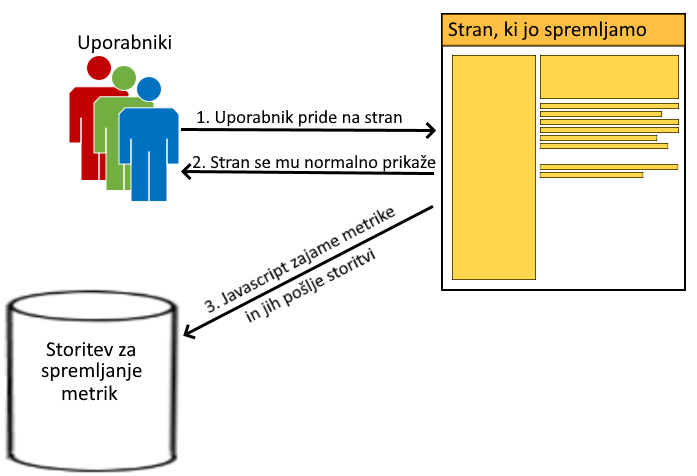
\includegraphics[width=0.9\textwidth]{rum_diagram.png}
	\end{center}
	\caption{Delovanje pasivnega spremljanja metrik}
	\label{img:rum}
\end{figure}

Ena od tehnologij pasivnega spremljanja je ti. spremljanje uporabniških metrik v realnem času (ang. Real User Monitoring, oziroma krajše RUM). S temi uporabniškimi metrikami, lahko nato zaznamo neželene pojave kot so pogoste napake ali upočasnitve. Zaznamo lahko odzivnost našega uporabniškega vmesnika, kjer spremljamo preklop med stanji aplikacije, pa tudi njegovo intuitivnost, tako, da spremljamo premik miške po zaslonu in vidimo, ali se uporabnik \sn{lovi} po zaslonu. Poleg tehničnih metrik, pa lahko spremljamo še ostale metrike, kot so število obiskov strani, ali se stranke vračajo na našo stran, kakšen čas v povprečju preživijo na njej, ipd.

Veliko teh metrik lahko spremljamo z uporabo orodij kot so Google Analytics \cite{ga_website} (nadalje GA), predvsem prej omenjene ne-tehnične metrike. GA je sicer orodje pisano za uporabo v klasičnih več-stranskih spletnih straneh, kjer se vsaka stran posebej naloži in takrat sproži dogodek, ki ga GA zabeleži, vendar lahko njegovo uporabo priredimo tako, da deluje tudi v aplikacijah na eni strani \cite{ga_spa}.

V primeru da želimo spremljati tehnične metrike naše aplikacije na eni strani, pa hitro ugotovimo, da nam GA ne zadošča. Tukaj je iniciativo prevzel Microsoft, z razvojem orodja Mezzurite \cite{mezzurite_website}, (v času izdelave diplomske naloge je bil v verziji 1) ki ponuja zbiranje metrik za ogrodja Angular \cite{angular_website}, AngularJS \cite{angularjs_website} in React \cite{react_website}.

Pri tem je Microsoft naletel na problem, da so navigacija in življenjski cikel aplikacije zelo odvisni od ogrodja, ki ga uporabljamo. Predstavili so rešitev, kjer so podprli samo tri ogrodja in v zameno olajšali delo razvijalcu, ki uporablja njihov produkt. Dolgih nosov so tako ostali razvijalci, ki uporabljajo npr. Vue.js (še eno izmed popularnih ogrodij). Ker pa se popularnost ogrodij in tehnologij zelo hitro spreminja, je pri takem pristopu treba biti neprestano obveščen o spremembah in jih poznati v globino. Ogrodje je potrebno poznati  precej dobro, da vemo kam umestiti naše spremljanje metrik. Tega se verjetno zaveda tudi Microsoft, saj je naznanil 2. verzijo Mezzurite platforme, kjer bo najverjetneje spremenil pristop.

Sam sem v zasnovi moje implementacije izbral drugačen pristop kot Microsoft. Zasnoval sem generično rešitev, ki deluje neodvisno od uporabljenega ogrodja. Ta zahteva nekaj več dela s strani razvijalca in razvijalec mora poznati ogrodje, ki ga uporablja. Hkrati pa mu to omogoča, da prilagodi spremljanje metrik tako, da mu bo dalo karseda točne metrike, primerne za njegovo aplikacijo.

\chapter{Razlike pri spremljanju metrik spletne aplikacije na eni strani (SPA) in klasične spletne strani}
\label{ch1}

Ker se aplikacije na eni strani razlikujejo v delovanju od klasičnih, se tako razlikuje tudi spremljanje metrik teh dveh pristopov. Merjenje metrik, je v tem primeru, potrebno prilagoditi drugačnemu načinu delovanja, da nam dajo bolj točne podatke. Nekatere od teh sprememb, pa potrebujejo tudi vpeljavo novih metrik, ki jih pri klasičnih straneh ne poznamo, saj pri SPA vplivajo na točnost rezultatov.

Pri prehodu iz klasičnih strani na SPA, pa se ne spremenijo samo metrike, ampak tudi njihova pomembnost. Klasične strani so večinoma pisane tako, da brskalnik prenese že zgrajeno stran in jo uporabniku samo prikaže, Javascript koda pa se samo odziva na dogodke, ki jih uporabnik proži – to so lahko kliki na gumb, ti. drag\&drop ali pa premik miške – in tako niso zahtevni za izvajanje. Pri SPA pa brskalnik prenese Javascript kodo, katera šele nato zgradi uporabniški vmesnik na odjemalčevi strani.

Izvajanje te kode pa se tukaj ne konča, saj velika večina teh ogrodij podpira tudi dvostransko vezavo podatkov (ang. two-way data binding). Torej, ko nek podatek v kodi zamenja vrednost (kot posledica rezultata AJAX klica, ali pa uporabniškega vnosa), se ta sprememba takoj pozna na vmesniku. Za dosego tega, je potrebno, da v ozadju koda neprestano posluša za spremembe ter da prepozna, kdaj je potrebno vmesnik na novo izrisati. S tem koda v naši aplikaciji ni več pasivna, ampak deluje aktivno. To odpre pot možnim puščanjem pomnilnika ali pa upočasnitvam aplikacije.

\begin{figure}[h]
	\begin{center}
		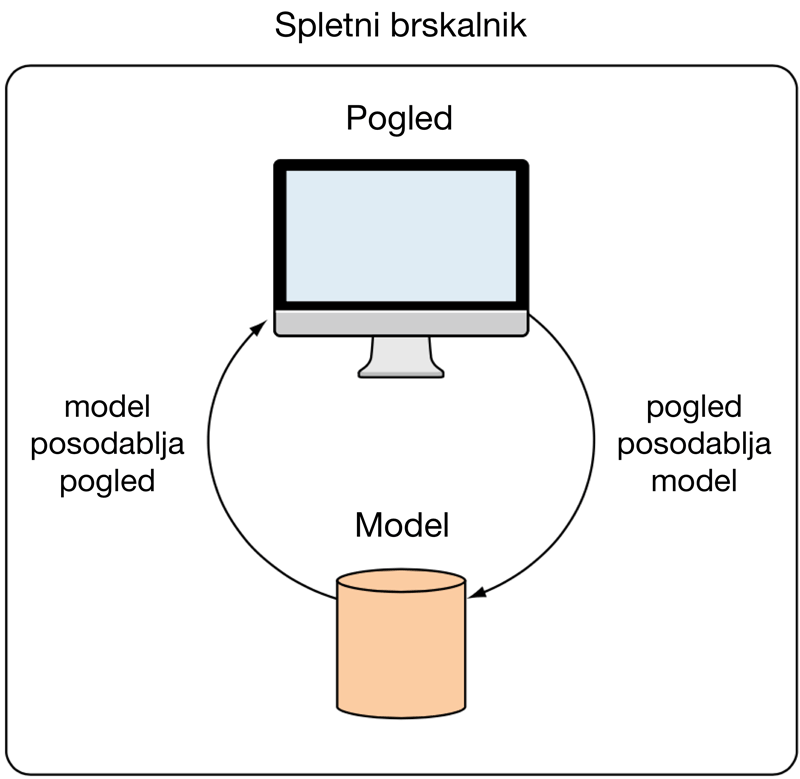
\includegraphics[width=0.9\textwidth]{AngularJS_dvosmerno_povezovanje.png}
	\end{center}
	\caption{Dvosmerno povezovanje pogleda in modela, vir: \cite{sp_skripta}}
	\label{img:angularjs_two_way_databind}
\end{figure}

Poveča se potreba po spremljanju metrik, saj imamo v bistvu tudi na odjemalcu precej kompleksen del naše aplikacije.

Ker je področje spremljanja metrik za SPA še precej novo, nimamo še poenotene terminologije za te metrike. Razne implementacije \cite{linkedin_rum}\cite{mezzurite_website} uporabljajo svojo terminologijo, vendar pa koncepti ostajajo isti.

Pri vseh implementacijah je moč najti zagonski čas aplikacije (ang. application load time, oziroma krajše ALT). To je metrika, ki nam pove, koliko časa potrebuje naša aplikacija, da prenese zahtevane gradnike, naloži kodo ogrodja, ki ga uporabljamo in inicializira aplikacijo. Gre za precej pomembno metriko, saj če je zagonski čas predolg, lahko izgubimo kakšnega potencialnega uporabnika. Občutek predolgega nalaganja se velikokrat zmanjša tako, da najprej prikažemo stran, ki uporabniku sporoči, da se stran nalaga – v večini primerov je to krog, ki se vrti, ali pa kakšna črta, ki se obarva glede na napredek (pomislimo na Gmail odjemalca, ki nas obvesti, da se aplikacija nalaga, nato pa prikaže vsebino) – ko smo pa prepričani, da je aplikacija naložena, to stran skrijemo in prikažemo dejansko vsebino. Eden izmed načinov je tudi ta, da se poslužimo delnega strežniškega upodabljanja (ang. server-side rendering), tj. da stran delno izrišemo že na strežniku.

Naslednja omembe vredna metrika se uporablja že pri klasičnih straneh. To je čas nalaganja strani (ang. page load time, oziroma krajše PLT). Pri klasičnih aplikacijah je to najpogostejša metrika, ki nas zanima, saj nam pove, kako hitro uporabnik vidi vsebino te strani. Toda, ko skušamo to metriko vpeljati tudi v SPA, pridemo hitro do nekaj vprašanj, s katerimi se nismo srečali pri klasičnih straneh. Prvo vprašanje, ki se nam zastavi je, kdaj se stran sploh smatra za naloženo? Ali je to, ko se naloži DOM? Ali, ko se nam izriše vmesnik? Mogoče takrat, ko pridobimo podatke?

\begin{figure}[h]
	\begin{center}
		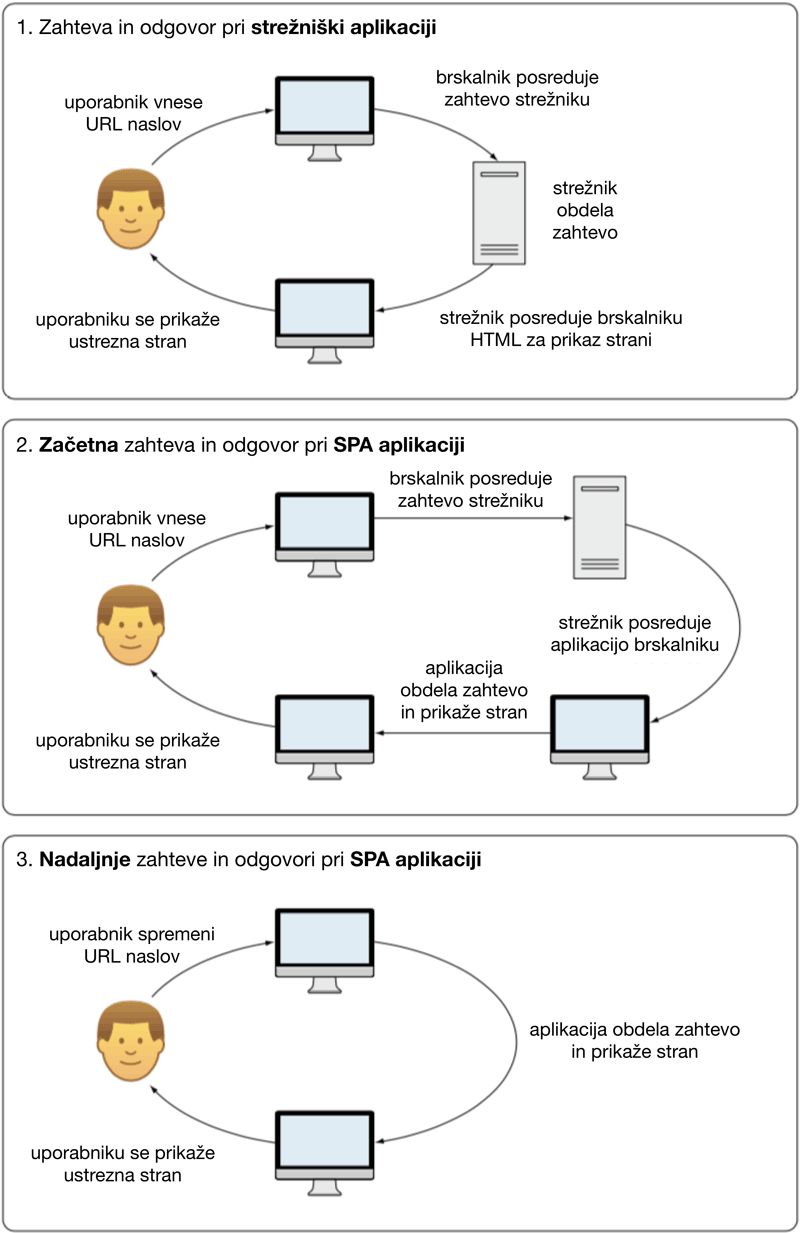
\includegraphics[width=0.9\textwidth]{Razlicni_nacini_obdelave_zahtev.png}
	\end{center}
	\caption{Različno delovanje SPA in klasičnih spletnih strani, vir: \cite{sp_skripta}}
	\label{img:diff_multipage_spa}
\end{figure}

Pravega odgovora ni, saj to povsem zavisi kako smo stran zasnovali. Tudi podatke, ki jih pridobivamo dinamično z AJAX zahtevki, ne obravnavamo z enako prioriteto. Podatki, ki gradijo osnovni pogled, na primer tabelo, so najverjetneje sestavni del strani in morajo biti zajeti v času nalaganja strani, medtem ko podatek, ki nam prikazuje število neprebranih sporočil v orodni vrstici ni bistven in ga lahko iz te metrike izpustimo. V tem primeru mora razvijalec sam presoditi, kdaj je stran uporabna in se smatra kot naložena.

Poleg že prej navedenega, pa je razlika tudi v navigaciji. Ali je ta stran prva, ki smo jo odprli, ali ena izmed sledečih? Namreč, kot je bilo že omenjeno, SPA se poslužujejo mehke navigacije. To je navigacija, ki spremeni url naslov in stanje zgodovine brskalnika z uporabo HTML5 history API-ja, brez, da bi se stran dejansko naložila. Posledica tega je, da je z izjemo prve, vsaka naslednja navigacija bistveno hitrejša. Torej če ne razlikujemo prve, \sn{trd} navigacije od ostalih, lahko hitro dobimo napačne podatke.

V čem pa se prva navigacija pravzaprav razlikuje od ostalih? Tukaj se spomnimo prej omenjenega zagonskega časa aplikacije. Ob prvi navigaciji, se morajo prenesti gradniki aplikacije, in nato se mora aplikacija inicializirati. Prva navigacija je sestavljena iz zagonskega časa aplikacije in časa nalaganja strani.

Zaradi tega dejstva, hitro opazimo, da uporaba imena PLT pri SPA ni primerna. PLT pri klasičnih aplikacijah vsebuje tudi čas, ki ga porabimo da prenesemo gradnike strani, v primeru mehke navigacije, pa teh gradnikov ne prenašamo. To se zgodi samo v zagonskem času aplikacije. Zato je tukaj primernejše govoriti o času nalaganja pogleda oziroma VLT (View Load Time). Prva navigacija je tako sestavljena iz dveh metrik, vsaka nadaljnja pa le iz ene.

Pri večini SPA ogrodij pa so strani v bistvu samo komponente. Tako bi lahko to metriko posplošili v čas nalaganja komponente (ang. component load time, oziroma krajše CLT). Čeprav VLT in CLT izgledata kot, da merita isto stvar, pa vendar obstaja razlika med njima. VLT se prične meriti, ko se navigacija začne. V vsakem ogrodju je to drugače implementirano, ampak običajno se navigacija začne, ko smo še na prejšnji strani. V VLT tako zajamemo tudi čas, ki ga ogrodje porabi, da razreši katero komponento mora prikazati za zahtevan url.

Komponenta pa lahko pomeni tudi vnosno polje za datum -- ta komponenta ne bo imela svojega URL-ja, in bo lahko uporabljena na več straneh, ali pa celo večkrat na eni strani. Tukaj nas navigacija pravzaprav ne zanima, zanima nas samo koliko časa potrebuje komponenta, da se instancira in postane uporabna. Namesto na navigacijo, se tukaj zanašamo na življenjski cikel komponente. Vsaka komponenta ima, odvisno od ogrodja, definiran življenjski cikel, kjer se ustvari instanca komponente, izriše njen pogled, pridobi podatke, ki jih komponenta potrebuje in kjer se ta instanca izbriše iz spomina, ko je ne potrebujemo več.

To metriko je smiselno uporabiti na bolj kompleksnih komponentah, oziroma ti. \sn{pametnih} komponentah, ki znajo podatke pridobivati in obdelovati, da tako spremljamo njihovo učinkovitost. Pri \sn{neumnih} komponentah, tistih, ki znajo podatke samo prikazati, ne pa tudi pridobiti, pa najverjetneje ni.

\chapter{Zajete metrike}
\label{ch2}

Metrik, ki jih lahko spremljamo pri spletnih aplikacijah je veliko. Prav zaradi tega sem se pri svoji implementaciji osredotočil le na nekaj izbranih metrik, ki dobro predstavijo proces zbiranja metrik. Večina teh metrik je formalne narave, kjer ima metrika številčno vrednost in lahko na njej opravljamo statistično analizo. Tako lahko vidimo, ali prihaja do problemov pri večjem deležu uporabnikov, ali pa le pri peščici.

Danes imamo namreč veliko spletnih standardov, ki jih ne podpirajo vsi brskalniki. To je sploh očitno pri uporabi starejših brskalnikov. Če iz zbranih podatkov razberemo, da ima nek določen problem samo peščica ljudi in to zaradi starejšega brskalnika, je mogoče cenejše opustiti podporo za ta brskalnik, kot pa prilagoditi aplikacijo zanj. Nedavno smo bili priča takemu primeru, ko je eden od popularnejših ponudnikov GIT repozitorijev, GitHub, sporočil novico, da so opustili podporo za Internet Explorer [Slika \ref{img:github_ie}]

\begin{figure}[h]
	\begin{center}
		
\includegraphics[width=1\textwidth]{github_end_support.png}
	\end{center}
	\caption{Obvestilo na GitHub strani, odprti z Internet Explorer}
	\label{img:github_ie}
\end{figure}

Spremljamo pa lahko tudi metrike neformalne narave, kjer podatki nimajo neke številčne vrednosti, oziroma nam ta vrednost ne predstavlja neke dodane informacije. Tak primer je zajemanje premikov miške, kjer vidimo, kako intuitiven je naš vmesnik za uporabnika. Statistična analiza na teh podatkih nam ne bi prinesla ravno uporabnih podatkov, saj formula ne more vedeti, kako je naš uporabniški vmesnik zasnovan. V tem primeru, je veliko bolj smiselno podatke evaluirati vizualno.

\section{Zagon aplikacije}
\label{ch2:sec1}
Kot je bilo že prej omenjeno, nam ta metrika pove koliko časa potrebuje naša aplikacija od trenutka ko v naslovno vrstico vnesemo spletni naslov aplikacije in pritisnemo ENTER, pa do prve navigacije na naši strani. Za označbo te metrike se uporablja angleška kratica ALT – Application Load Time.

Metriko zajemamo s pomočjo HTML5 performance API-jem. Ta API nam izpostavi začetni čas navigacije, tj. ko smo pritisnili tipko ENTER, oziroma kliknili na povezavo, ki kaže na našo aplikacijo. Ta začetni čas pridobimo s klicem \verb|performance.timing.navigationStart| (uporaba v opuščanju) oziroma, z novejšim \verb|performance.timeOrigin|. Vse kar mora razvijalec narediti, da prične beležiti metriko je, da na primernem mestu pokliče metodo \\ \verb|MetricsMonitor.logApplicationStartup()|, ki zabeleži trenutni čas, tj. konec zagona aplikacije in ta podatek posreduje naši spletni storitvi, ki ta podatek shrani.

\begin{lstlisting}[label=app_startup_report, caption=Poročilo zagonskega časa aplikacije]
{
  "minLoadTime": 124,
  "maxLoadTime": 2616,
  "avgLoadTime": 417.30232558139534,
  "percentiles": [
    {
      "percentile": 0.95,
      "value": 1598.6999999999985
    }
  ]
}
\end{lstlisting}

Ob zadostnem številu zbranih podatkov, si lahko ogledamo poročilo zagonskega časa, ki ga storitev izpostavi preko REST API-ja.


\section{Čas nalaganja pogleda}
\label{ch2:sec2}

Čas nalaganja pogleda, je čas, ki ga aplikacija porabi od klika na povezavo, do trenutka, ko vidimo vsebino zahtevane strani. Kaj se smatra kot vsebino strani je subjektivno, saj se to razlikuje od aplikacije do aplikacije. V takem primeru je to odločitev najbolje prepustiti razvijalcu, saj najbolje pozna aplikacijo. Za označbo te metrike se uporablja kratica VLT – View Load Time.

Posebej je potrebno izpostaviti čas nalaganja prvega pogleda (ang. first view load time, oziroma krajše FVLT). Ta čas dobimo tako, da seštejemo zagonski čas aplikacije in čas nalaganja pogleda.

\begin{equation}
\label{eq-01}
FVLT = ALT + VLT
\end{equation}

Pomembno je, da ko merimo hitrost nalaganja posamezne strani (z VLT metriko), pri tej ne upoštevamo FVLT, saj tako lahko pokvarimo zajete podatke. Če na to nismo pozorni, se lahko hitro zgodi, da nam metrika pokaže, da je naša naslovna stran najpočasnejša, kar pa ni vedno res, lahko je le najpogostejša stran, ki jo uporabnik prvo obišče.

Za beleženje te metrike ne potrebujemo nobenega posebnega HTML5 API-ja, saj se metrika zajema, ko je DOM že v celoti naložen in nam tako standarden \verb|Date| objekt povsem zadostuje. Razvijalec v tem primeru uporabi dve metodi in sicer \verb|MetricsMonitor.logPageLoadStart(url)| in \\ \verb|MetricsMonitor.logPageLoadEnd(url)|. Metrika se shranjuje pod unikatnim imenom, da jo lahko razberemo od ostalih. Za unikatno ime je priporočljivo uporabiti kar url strani. Isto metodo pa lahko uporabimo tudi za merjenje CLT posamezne komponente – tam uporabimo neko drugo, smiselno ime.
 
Enako kot pri zagonskem času aplikacije, nam storitev izpostavi poročilo te metrike preko REST vmesnika.

\begin{lstlisting}[label=page_load_report, caption=Poročilo časa nalaganja pogleda]
{
  "pages": [
    {
      "pathname": "/",
      "minLoadTime": 25,
      "maxLoadTime": 341,
      "avgLoadTime": 69.04347826086956,
      "pageHits": 23,
      "percentiles": [
        {
          "percentile": 0.95,
          "value": 120.1
        }
      ]
    },
    {
      "pathname": "/service/{id}",
      "minLoadTime": 26,
      "maxLoadTime": 295,
      "avgLoadTime": 72.18518518518519,
      "pageHits": 27,
      "percentiles": [
        {
          "percentile": 0.95,
          "value": 212.49999999999997
        }
      ]
    }
  ],
  "averagePageLoadTime": 69.43939393939394
}
\end{lstlisting}

Poročilo nam za vsako stran izpiše minimalni, maksimalni in povprečni čas nalaganja, število kolikokrat je bila ta stran obiskana in percentile, ki jih lahko poljubno specificiramo s parametri zahtevka. Storitev ponuja še en dodatni parameter, s katerim lahko povemo storitvi naj v poročilo vključi tudi FVLT, ne samo VLT.

V poročilu \ref{page_load_report} pričakovano dobimo zelo kratke čase nalaganja pogleda, saj je navigacija v aplikacijah na eni strani precej hitra.

\section{Čas nalaganja gradnikov strani}
\label{ch2:sec3}

Velik delež zagonskega časa aplikacije normalno predstavlja nalaganje gradnikov strani. To so datoteke, ki jih naša aplikacija nujno potrebuje za svoje delovanje in so lahko različnega tipa, najpogosteje pa s tem mislimo na HTML, Javascript in CSS datoteke.

To metriko je smiselno spremljati zato, da lahko zaznamo ali imajo uporabniki težave s prenašanjem naše aplikacije. Seveda je prenos aplikacije odvisen od kvalitete internetne povezave našega uporabnika, to pa je faktor na katerega nimamo vpliva.

V kolikor prepoznamo, da ima znaten del naših uporabnikov težave s prenašanjem, se poslužimo raznih tehnik, ki naredijo našo aplikacijo bolj vitko. V kombinaciji z ostalimi metrikami, lahko zaznamo, da določena sekcija naše aplikacije ni tako obiskana kot ostale, recimo urejanje profila. Tako sekcijo je zato smiselno naložiti s ti. lenim nalaganjem, s čimer zmanjšamo zagonski čas aplikacije.

Za zajem te metrike se spet poslužimo HTML5 performance API-ja. Ob zagonu aplikacije, se sproži koda, ki z klicem \\ \verb|performance.getEntriesByType("resource")| odčita čase nalaganja posameznega gradnika ter njegovo velikost. Posamezen gradnik ima več časov nalaganja. API nam izpostavi čase preusmeritve, DNS razrešitve, vzpostavitve TCP povezave, SSL/TLS rokovanja. Iz izpostavljenih lastnosti, pa lahko izračunamo še začetek zahtevka in konec odgovora, iz katerega lahko dobimo celoten čas prenosa.

Velikost prenosa je tudi ena izmed metrik, ki jih API izpostavi, iz česar vidimo, kako velika datoteka se je dejansko prenesla. Pri testiranju te metode, sem pa opazil, da je velikost pogosto 0. To gre pripisati brskalnikovemu predpomnjenju teh gradnikov. Pri zajemanju te metrike, je tako smiselno izpustiti predpomnjene datoteke, saj se te niso prenašale in bi nam z ničelno vrednostjo pokvarile pravo sliko velikosti prenosa.

Ta metoda ima en pomemben predpogoj in sicer mora strežnik, ki streže te datoteke implementirati glavo HTTP zahtevka Time-Allow-Origin, kjer za vrednost podamo domene, iz katerih je zbiranje te metrike dovoljeno. Delovanje je tako podobno CORS-u.

Tudi pri tej metriki, nam storitev izpostavi poročilo preko REST vmesnika.

\begin{lstlisting}[label=resource_load_report, caption=Poročilo časa nalaganja gradnikov strani]
{
  "resources": [
    {
      "name": "http://192.168.1.22:32772/styles.6b7abb61d8006c2e7e17.css",
      "type": "link",
      "payloadSize": {
        "average": 245425.0,
        "minimum": 245425,
        "maximum": 245425
      },
      "requestSize": {
        "average": 52837.78571428572,
        "minimum": 224,
        "maximum": 245755
      },
      "requestTime": {
        "average": 39.035714285714285,
        "minimum": 2,
        "maximum": 562
      }
    },
    {
      "name": "http://192.168.1.22:32771/main.86563ff2a46d83c7aa1d.js",
      "type": "script",
      "payloadSize": {
        "average": 1642994.0,
        "minimum": 1642994,
        "maximum": 1642994
      },
      "requestSize": {
        "average": 1643339.0,
        "minimum": 1643339,
        "maximum": 1643339
      },
      "requestTime": {
        "average": 218.5,
        "minimum": 163,
        "maximum": 326
      }
    }
  ]
}
\end{lstlisting}

Poročilo nam za vsak gradnik posebej izpiše njegov tip, minimalno in maksimalno ter povprečno vrednost za tri metrike: velikost datoteke, velikost HTTP zahtevka (ki poleg datoteke vsebuje še meta podatke kot so HTTP glave -- ang. HTTP headers) in čas, ki je bil potreben, da se je datoteka prenesla.

\section{Sledenje premikov miške uporabnika}
\label{ch2:sec4}

Sledenje premikov miške je še zadnja od zajetih metrik. Za razliko od preostalih, nam ta ne meri hitrosti naše aplikacije, ampak jo uporabljamo, da ugotavljamo intuitivnost našega uporabniškega vmesnika. Ker ni formalne narave, ne moremo podatkov spraviti v neko številsko obliko in jih prikazati v poročilu, kot smo to storili s prejšnjimi metrikami.

Seveda, pa to ne pomeni, da so taki podatki nekoristni. Če te podatke konsolidiramo v skupine pikslov (npr. 20px X 20px), lahko za vsako tako skupino beležimo ti. vročinsko stopnjo. Ta stopnja nam predstavlja število kolikokrat je uporabnik šel z miško čez to skupino pikslov. Skupine pikslov, ki so okoli gumbov bodo tako imele višjo vročinsko stopnjo, kot tiste v robovih aplikacije, kjer običajno ni vsebine.

Ko imamo izračunane vročinske stopnje, lahko s temi stopnjami izrišemo vročinski zemljevid naše aplikacije. Za izris zemljevida, moramo spremeniti način delovanja odjemalca iz zajemanja metrik v risanje vročinskega zemljevida. Odjemalec bo tako pridobil podatke potrebne za izris, in jih izrisal na zaslon poleg naše aplikacije, kot je to vidno na sliki \ref{img:heatmap}. Pri tem bodo polja z višjo vročinsko stopnjo obarvana temnejše (rdeče), polja z nižjo pa svetlejše (zeleno).

\begin{figure}[h]
	\begin{center}
		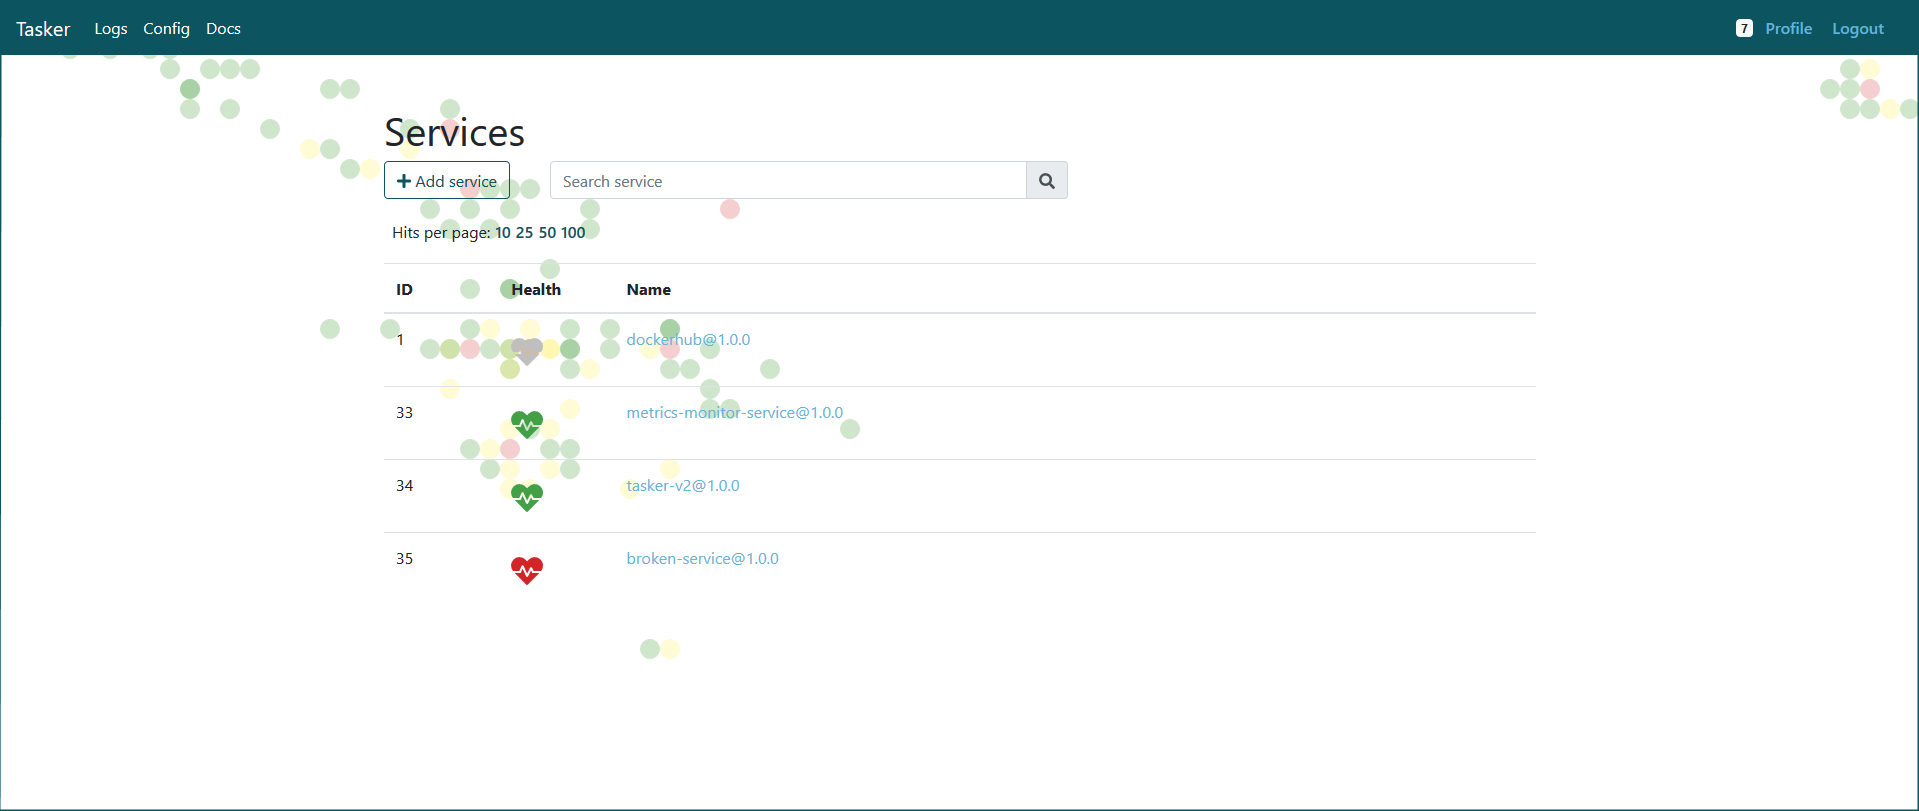
\includegraphics[width=1\textwidth]{heatmap_1.png}
	\end{center}
	\caption{Primer vročinskega zemljevida}
	\label{img:heatmap}
\end{figure}

Iz izrisanega vročinskega zemljevida lahko na neformalen način vidimo, ali se naši uporabniki preveč \sn{lovijo} po zaslonu, iz česar lahko sklepamo, da naš uporabniški vmesnik ni intuitiven. Vidimo pa lahko tudi množice najpogostejših akcij, ki jih uporabnik izbere. Če so gumbi za te akcije preveč oddaljeni med seboj, bo tako vročinski zemljevid izrisal pot med njimi, kar nam da informacijo, da je mogoče smiselno te gumbe premakniti bližje drug drugemu.

\section{Dodatne metrike}
\label{ch2:sec5}
V tem poglavju, bi rad izpostavil še nekaj metrik, ki niso bile vključene v prototip, bi jih pa bilo v nadaljnjem razvoju smiselno dodati zaradi njihove uporabnosti.

To so sledeče metrike:

\begin{description}
	\item[CLT:] O času nalaganja komponente sem govoril že v poglavju \ref{ch1}.
	\item[Beleženje poljubnih dogodkov:] S tem zajamemo poljubne enkratne dogodke, kot so recimo izvedba neke akcije ali pa odpiranje zunanje povezave, kar nam da večji vpogled v to, zakaj naši uporabniki uporabljajo našo aplikacijo.
	\item[Spremljanje vračanja strank:] S hrambo stanja v internetnih piškotkih, lahko spremljamo kolikokrat je uporabnik že obiskal našo stran iz neke naprave. Iz teh podatkov lahko sklepamo,  ali se stranke vračajo na našo stran. V primerih, ko imamo v aplikacijo vključeno še avtentikacijo, lahko spremljamo ali naši uporabniki dostopajo do aplikacije z različnimi napravami.
	\item[Spremljanje uporabniških naprav:] Velikokrat je smiselno spremljati tudi velikost zaslona in brskalnik. Tako lahko vidimo ali naši uporabniki pretežno uporabljajo mobilne naprave za dostop do aplikacije, kar pomeni, da moramo posvetiti več pozornosti odzivnemu uporabniškemu vmesniku.
	\item[Spremljanje časa uporabnika na strani:] Smiselno je beležiti tudi čas, ki ga uporabnik porabi na določeni strani. To še posebej drži za strani, katerih glavna funkcionalnost je prikazovanje vsebine, naprimer razne novičarske strani, blogi ali forumi. Čeprav je veliko takih strani pisanih še kot klasične strani, pa so nekatere že pisane tudi kot aplikacije na eni strani. Spletni portal 24ur.com tako uporablja Angular ogrodje za prikaz novic. Obstajajo pa tudi razni generatorji statičnih strani, ki generirajo vsebino, posredujejo pa jo kot aplikacijo na eni strani, dva popularnejša sta Gatsby \cite{gatsby_website} in VuePress \cite{vuepress_website}. V kombinaciji s prej omenjenim beleženjem dogodkov, lahko dobimo res dobro sliko o kvaliteti naše storitve, ki jo uporabnikom ponujamo kot našo aplikacijo.
	\item[Spremljanje uporabnikove lokacije] Spremljanje od kod naši uporabniki dostopajo do aplikacije je tudi zelo pomembno. V primeru, da so naši strežniki preveč oddaljeni od naše glavne baze uporabnikov, jih je smiselno postaviti bližje.
\end{description}

\chapter{Zasnova generične rešitve za zbiranje in spremljanje uporabniških metrik}
\label{ch3}

\section{Načrt}
\label{ch3:sec1}

Pri snovanju rešitve za zbiranje uporabniških metrik v realnem času, moramo biti še posebej pozorni, da z zbiranjem metrik ne poslabšamo uporabniške izkušnje naših uporabnikov. Pri takem zbiranju podatkov, je lahko uporabnikov aplikacije zelo veliko. Če se naša storitev, ki metrike shranjuje, ne obnese dovolj dobro pri velikem številu zahtevkov, potem to lahko upočasni našo aplikacijo, katere metrike spremljamo.

Naših uporabnikov pa te metrike ne zanimajo, njih zanima samo storitev, ki jo naša aplikacija ponuja.  V takem primeru, bodo uporabo naše aplikacije opustili in odšli h konkurenci. Najboljša rešitev za spremljanje metrik je torej taka, za katero uporabnik ne ve, ne da bi prebral ustrezna obvestila (opozorilo na piškotke in nova GDPR določila).

Metrike zajema knjižnica, ki jo vključimo v aplikacijo, katero želimo spremljati. Ta knjižnica odpre povezavo s storitvijo preko WebSocket protokola. Povezava se tako vzpostavi samo enkrat in ostane odprta dokler uporabnik uporablja aplikacijo. Preko te povezave nato pošiljamo zajete metrike. Nekatere metrike, kot so časi nalaganja se prenesejo takoj, medtem ko se premiki miške shranjujejo v medpomnilnik in se na vsakih nekaj zapisov prenesejo v storitev, da tako zmanjšamo število poslanih sporočil. Ko ta sporočila prispejo na strežnik, jih ta takoj umesti v sporočilno vrsto.

Iz tega razloga, sem v zasnovo vključil Apache Kafko, platformo za distribuirano pretakanje. V storitvi prevzema vlogo sporočilne vrste in s tem omogoča kasnejše procesiranje prejetih metrik. Drugi del storitve jemlje sporočila iz vrste in jih glede na njihov tip ustrezno procesira ter shrani v podatkovno bazo. Ta del je lahko počasnejši, saj na delovanje spremljane aplikacije nima vpliva. Če se izkaže, da sprejemanje in procesiranje sporočil v isti storitvi slabo vpliva na optimalno delovanje storitve, se lahko to storitev loči na dva dela. Ima pa storitev še tretjo komponento in to je generiranje poročil o zajetih metrikah. Ta del storitve, združi shranjene podatke in jih v JSON obliki posreduje razvijalcu.

\begin{figure}[h]
	\begin{center}
		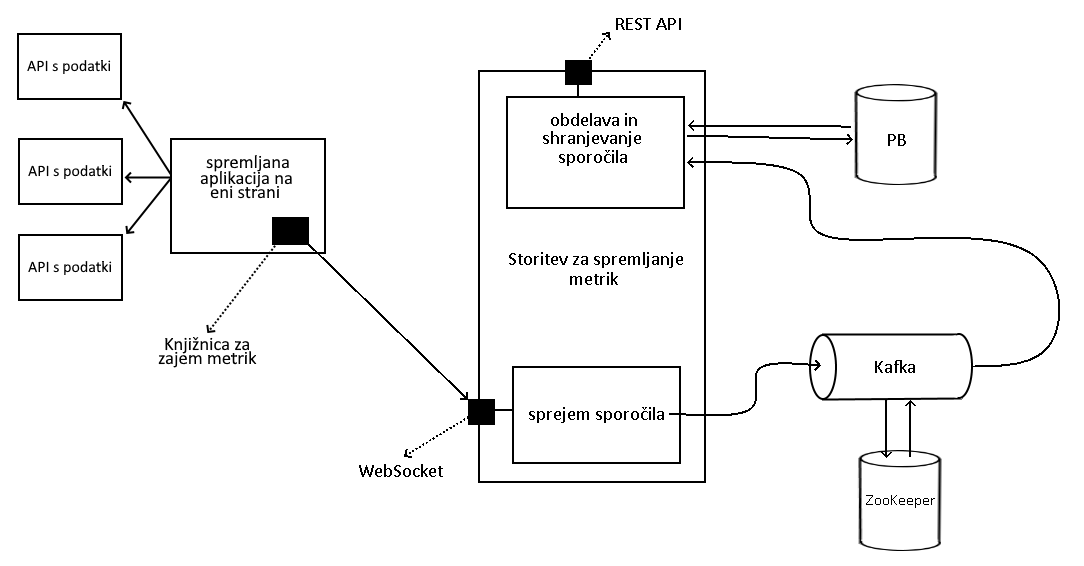
\includegraphics[width=1\textwidth]{design.png}
	\end{center}
	\caption{Načrt platforme}
	\label{img:design}
\end{figure}

Cilj te naloge je bil izdelati generično rešitev. Torej rešitev, ki je neodvisna od (ne)uporabljenega ogrodja. Da bi rešitev bila res generična se pri implementaciji knjižnice za zajem metrik, nisem poslužil nikakršnih optimizacijskih trikov, ki jih ogrodja prinašajo.

V drugem poglavju omenjen Mezzurite, je naredil prav to. Izkoristili so poznavanje delovanja ogrodja, tako, da so napisali knjižnico, ki posluša dogodke v življenjskem ciklu in izvaja beleženje ob primernih trenutkih. Ker pa taka rešitev ni generična, sem sam izbral drugačen pristop.

V svoji knjižnici tako samo izpostavim metode katere, mora razvijalec ustrezno umestiti v aplikacijo. Torej mora te poslušalce dogodkov sam implementirati, iz česar sledi, da mora tudi poznati življenjski cikel ogrodja, ki ga uporablja.

Pri shranjevanju podatkov o metrikah pa je izstopalo shranjevanje premikov miške, saj je teh podatkov lahko zelo veliko. Pri Full HD zaslonu imamo 1920 x 1080 pikslov, zaradi česar bi hranjenje vsakega piksla pomenilo zelo veliko shranjenih vrstic. Za izris vročinskega zemljevida pa pravzaprav ne rabim podatkov natačnih na en piksel, saj so ugototovitve iz zemljevida neformalne narave. Zato, da se izognem temu problemu, sem piksle združeval v skupine 20x20 pikslov. S tem sem zmanjšal hranjeno mrežo iz 1920 x 1080 na 96 x 54¸, torej sem zmanjšal število hranjenih vrstic iz dobrih dveh milijonov na približno pet tisoč vrstic.

\section{Implementacija}
\label{ch3:sec2}

Za prototip generične rešitve, je bilo potrebno implementirati spletno storitev, ki metrike shranjuje in knjižnico, ki te metrike zajema in posreduje storitvi.

\subsection{Knjižnica}
\label{ch3:sec2:sub1}

Čeprav je Javascript še vedno edini jezik, ki ga brskalniki podpirajo, pa danes poznamo veliko načinov za pisanje spletnih aplikacij. Kot de facto standard za distribucijo spletnih aplikacij se uporablja ECMAScript 5 verzijo Javascripta. Ker je pa to zelo star standard, praktično noben razvijalec ne uporablja več te verzije. Tako je najpogostejši proces tak, da pišemo našo aplikacijo v novejši verziji Javascripta (ta je trenutno ES10, oziroma ECMAScript 2019), nato pa uporabimo prevajalnik (ang. transpiler), ki prevede kodo na starejšo verzijo. Najpopularnejši Javascript prevajalnik je trenutno Babel.

Ni pa to edini način, ki se danes uporablja za razvoj aplikacij. Microsoft je razveselil velik del razvijalcev, ko je zasnoval TypeScript, jezik enak Javascriptu, ki pa v koraku prevajanja preveri tudi podatkovne tipe spremenljivk in nam tako ponudi statično preverjanje tipov.

Ker imamo več različnih načinov razvoja, pa imamo tudi več načinov nalaganja modulov (oziroma datotek in knjižnic) v našo aplikacijo \cite{js_modules}. CommonJS, AMD in UMD so le eni izmed njih. UMD, ki je kombinacija prvih dveh, nam ponuja največjo fleksibilnost pri uporabi, zato sem se odločil napisati knjižnico v tem modulskem sistemu.

Knjižnico sem pisal v prej omenjenem Typescriptu, ker dokumentiranje tipov, ki ga Typescript ponuja, omogoča lažjo uporabo knjižnice. Dodaten plus predstavlja tudi dejstvo, da v primeru, ko  uporabnik knjižnice uporablja samo Javascript, znajo moderni urejevalniki prebrati definicijo tipov in tako boljše predlagati uporabo knjižnice uporabniku.

V primerih, ko knjižnico vključimo v aplikacijo z \verb|<script>| elementom, pa je pomembno tudi, da je ta knjižnica karseda majhna, da se hitreje naloži. Da to dosežemo se pri prevajanju izvede dodaten korak, minifikacija, ki kodo optimizira, odstrani neuporabljene dele kode in tako lahko zmanjša velikost knjižnice tudi za več kot 50\%.

Vse te korake sem avtomatiziral z uporabo orodja Webpack, ki preko vtičnikov omogoča izvedbo celotnega prevajalnega cikla z enim ukazom. 

Prevedeno knjižnico sem nato namestil v zaseben NPM repozitorij, gostovan na Sonatypovem Nexusu, od koder sem knjižnico nato prenašal, za uporabo v testnih aplikacijah.

\subsection{Storitev}
\label{ch3:sec2:sub2}

Storitev sem razvijal v platformi Open JDK Java 11, pri čemer sem uporabil spletno ogrodje KumuluzEE, ki implementira specifikacije JakartaEE (oz. JavaEE 8) in MicroProfile 2.2. Ogrodje je bilo sprva razvito kot rezultat diplomske naloge \cite{kumuluz_diploma}. Ena od prednosti uporabe tega ogrodja je ta, da našo kodo zapakira v eno samo JAR datoteko, pogosto imenovano Fat Jar oziroma Uber Jar. V to datoteko nam vključi tudi Jetty strežnik, kar nam precej olajša namestitev programa, saj nam ni potrebno konfigurirati aplikacijskih strežnikov, kot je JavaEE to včasih zahtevala, ampak se celoten program preprosto požene z ukazom \verb|java -jar server.jar|.

Prenašanje knjižnic od katerih je naša storitev odvisna, prevajanje izvorne kode in pakiranje vseh gradnikov v JAR datoteko, upravljamo z orodjem Apache Maven. To orodje je danes standard pri razvoju programov v Javi, uporablja pa se ga lahko tako z Enterprise, kot s standardno verzijo Jave.

Za komunikacijo s knjižnico naša storitev izpostavi dostopno točko za protokol WebSocket, preko katerega sprejema sporočila. WebSocket nam omogoča polno dvojno komunikacijo (ang. full-duplex) s strežnikom preko ene TCP povezave, s čimer zmanjšamo velikost in število povezav potrebnih za komunikacijo, v primerjavi z alternativo kot je recimo HTTP polling.

Prejeta sporočila storitev potiska v čakalno vrsto v Kafko. Apache Kafka je orodje, ki je zmožno obdelovati pretočna sporočila v realnem času, lahko pa se ga uporablja tudi kot sporočilno vrsto tipa objavi-naroči (ang. publish-subscribe). Za Kafko sem se odločil, ker zna, za razliko od RabbitMQ, obdelati večje število sporočil. Za prototipiranje sem uporabljal eno instanco Kafke, v realnih primerih pa imamo teh instanc več, saj tako lahko izkoristimo potencial Kafke kot distribuirano storitev. Kafka za svoje delovanje potrebuje tudi delujočo instanco ZooKeeperja, preko katerega Kafka obvešča o lokacijah vseh instanc.

Podatki se med komponentami platforme prenašajo kot JSON objekti, serializirani v niz. Tej nizi se  nato z uporabo Jackson knjižnice pretvorijo v Javanske objekte (POJO).

Deserializirani objekti se z uporabo JPA tehnologije zapisujejo v podatkovno bazo. Kot bazo bi načeloma lahko uporabili katerokoli transakcijsko bazo, odločil pa sem se za PostgreSQL 11, saj ima veliko vgrajenih funkcij za računanje statistike, katere uporabljam pri generiranju poročil.

Poročila, ki jih generiram s pomočjo teh SQL poizvedb pa so nato izpostavljena in dostopna razvijalcu preko REST vmesnika, ki posreduje poročilo v JSON obliki, kot je to vidno v izsekih kode \ref{app_startup_report}, \ref{page_load_report} in \ref{resource_load_report}.

\subsection{Podporne tehnologije}
\label{ch3:sec2:sub3}

Za namestitev moje storitve uporabljam orodji za virtualizacijo Docker in Docker Compose. Storitev se zapakira v JAR datoteko, nato pa uporabim to datoteko, da zgradim sliko vsebnika Docker. Ostali gradniki, od katerih je moja storitev odvisna -- Kafka, Zookeeper in PostgreSQL baza, so ravno tako prenešeni v obliki Docker slike.

Ker so gradniki tudi med seboj odvisni, moramo biti pozorni pri vrstnem redu zagona teh gradnikov. Proces lahko poenostavimo z uporabo orodja Docker Compose. To orodje nam omogoča, da izpostavimo odvisnosti med gradniki katere zna nato pognati v pravilnem vrstnem redu. Zgrajene slike se hranijo v privatnem Docker registru, ki je gostovan na istem Nexus strežniku, kot prej omenjen NPM repozitorij.

\section{Prototip}
\label{ch3:sec3}

Ugotovitve prejšnjih poglavij sem uporabil tako, da sem razvil prototip platforme, ki metrike sprejema, shranjuje in prikazuje. V naslednjem delu bom predstavil razviti izdelek in njegovo uporabo. Vsa koda, ki je bila razvita v procesu prototipiranja je objavljena na GitHub in javno dostopna na naslovu \url{https://github.com/Jamsek-m/diploma-thesis}.

\subsection{Namestitev}
\label{ch3:sec3:sub1}

Namestitev te platforme sestoji iz dveh delov: namestitev zalednega dela, tj. storitve, ki metrike hrani in knjižnice, ki metrike zajema.

\subsubsection{Zaledni del}

Zaledni del ima veliko deležnikov, zaradi tega se priporoča uporaba orodja Docker Compose, saj nam namestitev zelo olajša. Vse kar potrebujemo je spisati docker-compose.yml datoteko, katere primer vidimo spodaj.

\begin{lstlisting}[label=docker_compose, caption=Primer datoteke docker-compose.yml]
version: "3"
networks:
 metrics-net:
   name: metrics-net
services:
  postgres:
    image: postgres
    ports:
      - "5433:5432"
    environment:
      POSTGRES_USER: postgres
      POSTGRES_PASSWORD: postgres
      POSTGRES_DB: metrics-monitor
    networks:
      - metrics-net
  zookeeper:
    image: wurstmeister/zookeeper
    ports:
      - "2181:2181"
    networks:
      - metrics-net
  kafka:
    image: wurstmeister/kafka
    ports:
      - "9092:9092"
    depends_on:
      - zookeeper
    environment:
      KAFKA_ADVERTISED_HOST_NAME: localhost
      KAFKA_ZOOKEEPER_CONNECT: zookeeper:2181
    networks:
      - metrics-net
  metrics-monitor-service:
    image: metrics-monitor-service
    ports:
      - "8080:8080"
    depends_on:
      - kafka
      - postgres
    environment:
      KUMULUZEE_DATASOURCES0_CONNECTIONURL: jdbc:postgresql://postgres:5433/metrics-monitor
      KUMULUZEE_DATASOURCES0_USERNAME: postgres
      KUMULUZEE_DATASOURCES0_PASSWORD: postgres
      KUMULUZEE_STREAMING_KAFKA_PRODUCER_BOOTSTRAPSERVERS: kafka:9092
      KUMULUZEE_STREAMING_KAFKA_CONSUMER_BOOTSTRAPSERVERS: kafka:9092
    networks:
      - metrics-net
\end{lstlisting}

Ko imamo tako datoteko spisano, se preprosto z ukazno lupino premaknemo v direktorij, kjer se ta datoteka nahaja in vpišemo ukaz \verb|docker-compose up|.

Docker Compose bo prebral to datoteko, prenesel vse potrebne slike vsebnikov, jih pognal v ustreznem vrstnem redu (ki smo ga v datoteki definirali z uporabo \verb|depends_on|) in povezal v skupno omrežje, da bodo lahko med seboj komunicirali.

\subsubsection{Namestitev in uporaba knjižnice}

Knjižnico se v aplikacijo lahko vključi na dva načina. Prvi je klasični, kjer knjižnico naložimo kot Javascript datoteko z uporabo \verb|<script>| HTML elementa. Pri takem načinu uporabe je knjižnica dostopna preko globalnega objekta.

Drugi, priporočen način uporabe, je z namestitvijo knjižnice preko NPM-ja. To storimo s preprostim ukazom \verb|npm install --save metrics-monitor|. V takem primeru običajno uporabljamo kakšno orodje kot je Webpack, saj knjižnico vključimo samo v Javascript kodo, to orodje pa nato zazna uporabo knjižnice in jo doda preostali kodi.

Naslednja demonstracija je vključitev knjižnice v aplikacijo, zgrajeno z Angular 8, katere koda je tudi dostopna na GitHubu.

\paragraph{Inicializacija aplikacije} 
Angular ob prvem zagonu kliče posebno metodo \verb|bootstrapModule()|, ki se nahaja v \verb|main.ts|.

\begin{lstlisting}[label=lib_main_ts, caption=Zagon Angular aplikacije]
if (environment.production) {
  enableProdMode();
}

platformBrowserDynamic().bootstrapModule(AppModule)
  .catch(err => console.error(err));
\end{lstlisting}

Tukaj moramo dodati inicializacijsko kodo za našo knjižnico. Metodi je treba dodati še nekaj parametrov in sicer URL naslov storitve, ki shranjuje metrike, način delovanja in ime aplikacije za razločevanje v primerih ko spremljamo metrike več aplikacij. \\

\begin{lstlisting}[label=lib_main_ts_after, caption=Inicializacija knjižnice]
if (environment.production) {
  enableProdMode();
}

MetricsMonitor.init({
  applicationName: "angular-sample",
  mode: "capture",
  serverUrl: "http://localhost:8080",
  log: "debug",
  urlsWithParameters: [
    "/service/{id}"
  ]
}).then(() => {
  platformBrowserDynamic().bootstrapModule(AppModule)
    .catch(err => console.error(err));
}).catch((err: Error) => {
  console.error(err);
});
\end{lstlisting}

Kot je razvidno iz kode \ref{lib_main_ts_after}, imamo še dva opcijska parametra: prvi je stopnja beleženja dnevnika -- ko razvijamo in testiramo aplikacijo je bolje imeti sporočila z več podrobnostmi, ki jih v produkciji raje ne prikazujemo.

Drugi parameter pa pride prav, ko imamo dinamične strani. To so strani, ki spreminjajo vsebino glede na URL parameter, obdržijo pa enako strukturo. Na sliki \ref{img:heatmap} vidimo seznam. Če kliknemo na katero izmed vrstic v seznamu, se nam odpre stran, ki prikazuje različne podatke glede na izbrano vrstico. Kar se spreminja je identifikacijski ključ elementa, ki določi katera vsebina se prikaže. Velikokrat je smiselno, da take strani združimo v eno, z uporabo ohranitvenika (ang. placeholder), kar nam uporaba tega parametra omogoča.

\paragraph{Zajem zagonskega časa aplikacije in začetka nalaganja pogleda}

To nastavimo v korenski komponenti (največkrat imenovani \verb|app.component.ts|).

\begin{lstlisting}[label=lib_app_comp, caption=Zajem zagonskega časa aplikacije in začetka nalaganja pogleda]
@Component({
  selector: "app-root",
  templateUrl: "./app.component.html",
  styleUrls: ["./app.component.scss"]
})
export class AppComponent implements OnInit {

  constructor(private router: Router) { }

  ngOnInit(): void {
    MetricsMonitor.logApplicationStartup();
    this.router.events.subscribe(routerEvent => {
      if (routerEvent instanceof NavigationStart) {
        MetricsMonitor.logPageLoadStart(routerEvent.url);
      }
    });
  }
}
\end{lstlisting}

Tukaj se poslužujemo znanja Angularjevega življenskega cikla in modula Router.

Ko se Angular komponenta inicializira, preveri ali ta komponenta implementira metodo ngOnInit() in jo izvede. Ker je to korenska komponenta aplikacije, pomeni, da se je naša aplikacija uspešno zagnala, zato na tej točki zabeležimo končni zagonski čas aplikacije.

S poznavanjem modula Router (iz knjižnice \verb|@angular/router|) pa lahko zajamemo čas pričetka nalaganja pogleda. Tukaj namreč poslušamo za dogodke, ki jih Router proži. V Angularju je eden od teh dogodkov NavigationStart, ki se sproži, ko uporabnik zahteva spremembo pogleda.

\paragraph{Zajem časa nalaganja pogleda}

Ko se zabeleži čas nalaganja pogleda, se na strežnik pravzaprav ne pošlje še noben podatek. Da se zabeleži čas nalaganja strani in se podatki pošljejo na strežnik, moramo poklicati še metodo za beleženje konca nalaganja pogleda. To postavimo na ustrezno mesto, ko je vsebina, pomembna za ta pogled naložena. Kaj je ustrezno mesto, pa zavisi od primera.

\begin{lstlisting}[label=lib_page_comp, caption=Zajem časa nalaganja pogleda]
@Component({
  selector: "app-first-page",
  templateUrl: "./first-page.component.html",
  styleUrls: ["./first-page.component.scss"]
})
export class FirstPageComponent implements OnInit, AfterViewInit {

  public displayedData: any[] = [];

  constructor(private router: Router, private dataService: DataService) { }

  ngOnInit() {
    // 1. primerno mesto:
    // ko se komponenta za pogled instancira
    MetricsMonitor.logPageLoadEnd(this.router.url);
  }

  ngAfterViewInit(): void {
    // 2. primerno mesto:
    // ko se pogled izrise na zaslon
    MetricsMonitor.logPageLoadEnd(this.router.url);
  }

  private getData(): void {
    this.dataService.getData().subscribe(
      data => {
        this.displayedData = data;
        // 3. primerno mesto:
        // ko pridobimo podatke,
        // ki so bistveni za prikaz strani
        MetricsMonitor.logPageLoadEnd(this.router.url);
      }
    );
  }
}
\end{lstlisting}

\paragraph{Zajem premikov miške}

Knjižnica ob inicializaciji registrira poslušalca dogodka premika miške. Ta poslušalec v ozadju beleži premike miške, jih shranjuje v medpomnilnik in, ko se ta napolni, posreduje strežniku. Razvijalcu tako za zajem te metrike ni potrebno storiti nič.

\section{Testiranje in poročila}
\label{ch3:sec4}

\subsubsection{Vročinski zemljevid}

Če hočemo iz vročinskega zemljevida kaj razbrati, moramo zemljevid projecirati na našo aplikacijo. To lahko storimo z zajemom zaslonskih mask na katere narišemo zemljevid, še boljši način pa je, da te podatke projeciramo kar v našo aplikacijo.

Knjižnica za zajem metrik ima dva načina delovanja. S prvim smo se že spoznali, ko smo zajemali metrike. Drugi način delovanja pa ne zbira metrik, ampak iz storitve pridobi podatke o premikih miške, katere nato projeciramo.

Za delovanje projeciranja, moramo spremeniti našo kodo na dveh lokacijah. Prva je pri inicializaciji knjižnice:

\begin{lstlisting}[label=heatmap_init, caption=Sprememba načina delovanja knjižnice]
MetricsMonitor.init({
  applicationName: "angular-sample",
  mode: "heatmap",
  serverUrl: "http://localhost:8080",
})
\end{lstlisting}

Ker pa ima vsaka stran svoj zemljevid, moramo še popraviti našo kodo tako, da se zemljevid na novo izriše, ko odpremo novo stran. To storimo s poslušanjem dogodkov Routerja, kot smo to počeli pri zbiranju časov nalaganja pogledov.

\begin{lstlisting}[label=heatmap_redraw, caption=Sprememba zemljevida ob prehodu na novo stran]
this.router.events.subscribe(routerEvent => {
  if (routerEvent instanceof NavigationEnd) {
    MetricsMonitor.redrawHeatmap();
  } else if (routerEvent instanceof NavigationStart) {
    MetricsMonitor.logPageLoadStart(routerEvent.url);
  }	
});
\end{lstlisting}

Ko je to storjeno, odpremo aplikacijo v brskalniku, kjer se nam bo izrisal zemljevid, kot je viden na slikah \ref{img:heatmap1} in \ref{img:heatmap2}.

\begin{figure}[h]
	\begin{center}
		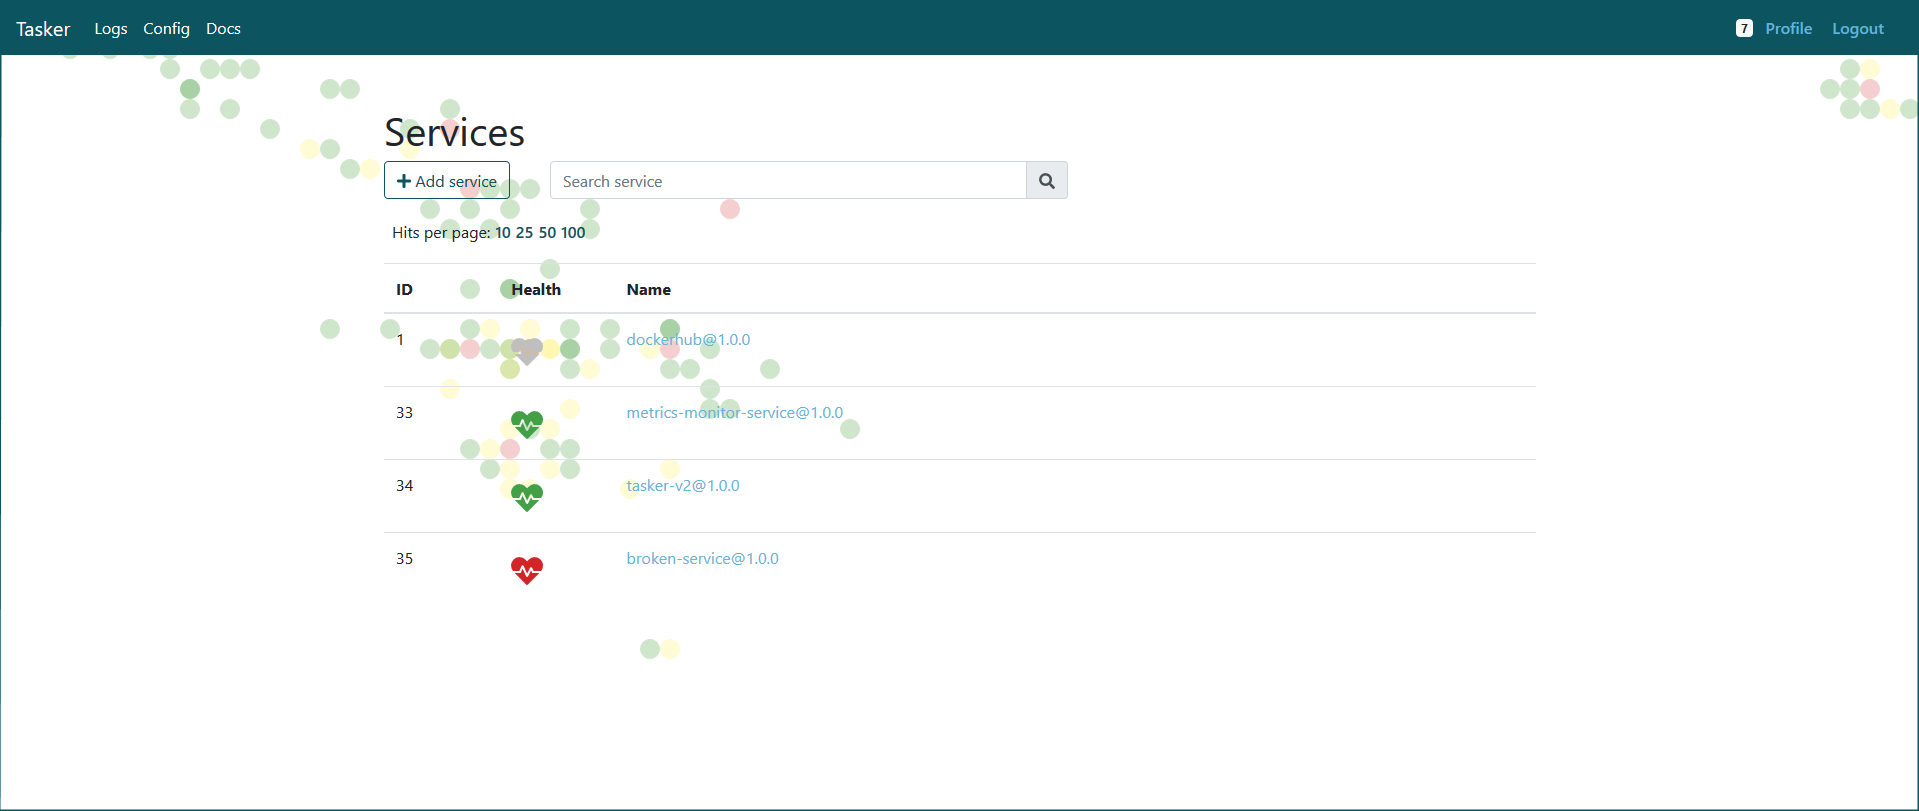
\includegraphics[width=1\textwidth]{heatmap_1.png}
	\end{center}
	\caption{Vročinski zemljevid za stran '/'}
	\label{img:heatmap1}
\end{figure}

\begin{figure}[h]
	\begin{center}
		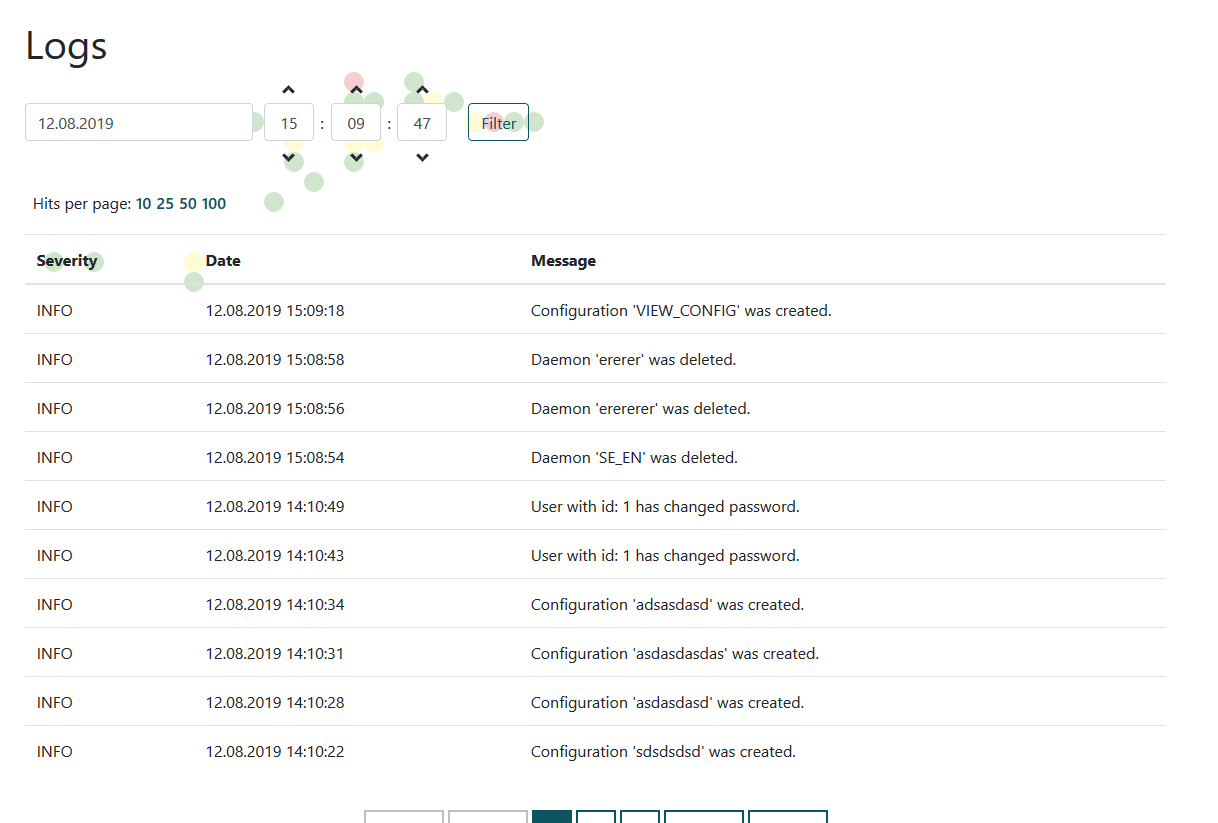
\includegraphics[width=1\textwidth]{heatmap_2.png}
	\end{center}
	\caption{Vročinski zemljevid  za stran '/logs'}
	\label{img:heatmap2}
\end{figure}

\subsubsection{Številske metrike}

Za ostale zajete metrike, ki so bolj formalne narave, imamo na voljo poročila (primeri vidni na \ref{app_startup_report}, \ref{page_load_report} in \ref{resource_load_report}).

Ta poročila lahko uporabimo za statistično analizo, s katero lahko ugotovimo, ali je naša aplikacija odzivna, ali se gradniki prenesejo iz strežnika dovolj hitro in če ne, na kolikšen del uporabnikov to vpliva.

\begin{figure}[h]
	\begin{center}
		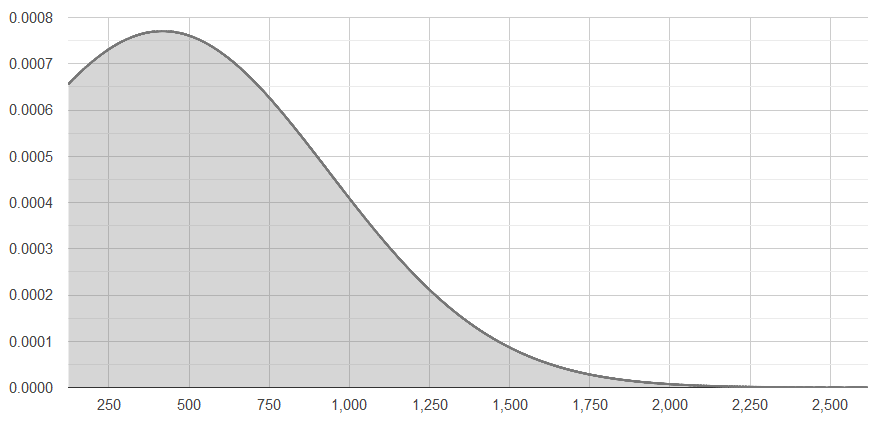
\includegraphics[width=1\textwidth]{app_startup_graph.png}
	\end{center}
	\caption{Zagonski časi aplikacije. Iz grafa razberemo, da se velikemu delu uporabnikov aplikacija zažene v približno 500ms, medtem, ko se majhnemu deležu uporabnikov aplikacija zažene v 1,5s ali več. Te številke potrdimo s pregledom poročila \ref{app_startup_report}.}
	\label{img:graph_app_startup}
\end{figure}

\begin{figure}[h]
	\begin{center}
		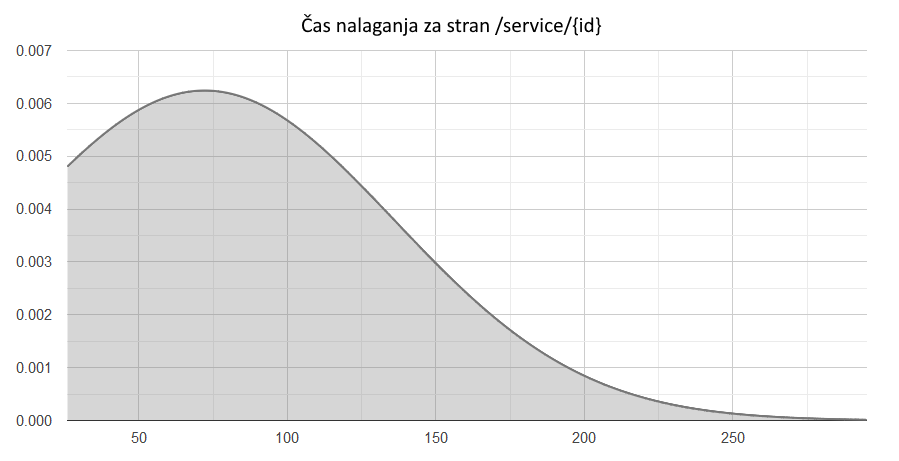
\includegraphics[width=1\textwidth]{page_load_graph_service_details.png}
	\end{center}
	\caption{Čas nalaganja pogleda '/service/:id'. Iz grafa razberemo, da se stran povečini naloži v 100ms, lahko pa tudi več, ampak ta čas ne presega 300ms, kar je precej dober čas.}
	\label{img:graph_page_load}
\end{figure}

Primeri grafov sicer uporabljajo podatke, ki so bili pridobljeni na precej majhni množici uporabnikov (n = 5). Pri tem sta dva uporabnika dostopala do aplikacije večkrat, saj so morale metrike zajeti tudi primere, ko so bile datoteke shranjene v predpomnilnik brskalnika.

V realnem primeru je naša množica uporabnikov veliko večja, zaradi česar so tudi podatki bolj točni in se oblikujejo v normalno porazdelitev.

\chapter{Sklepne ugotovitve}
\label{ch4}

Danes živimo v informacijski dobi. To pomeni, da so informacije postale ena izmed pomembnih surovin, ki jih podjetja potrebujejo za ustvarjanje dobička. Zajemanje metrik, opisanih v tej diplomski nalogi, je samo podmnožica vseh informacij, ki se zbirajo o nas. Če so to do včeraj počela samo FAANG/FAAMG podjetja (Facebook-Amazon-Apple-Netflix-Google oziroma Facebook-Amazon-Apple-Microsoft-Google), pa danes to počnejo tudi že veliko manjša podjetja. Zajemanje metrik bo tako samo še naraščalo v svoji pomembnosti in popularnosti.

Tega se zavedajo tudi razvijalci brskalnikov in sodelavci W3C, saj se HTML5 APIji za merjenje metrik neprestano posodabljajo, spreminjajo in izboljšujejo. V času pisanja diplome se specifikacije APIjev šele oblikujejo in so še daleč od standardiziranega načina uporabe. V zasnovi so tako specifikacije za spremljanje pasovne širine uporabnika, spremljanje porabe energije na napravi ter še marsikaj drugega. Brskalniki jih trenutno vključujejo kot eksperimentalne funkcionalnosti, ki so lahko stvar spremembe. Za nekatere implementacije tudi velja, da ne delujejo še zanesljivo.

Iz tega razloga je smiselno počakati na konec zasnove specifikacije preden začnemo tako metriko spremljati. Velikokrat nam lahko napačno zajeta metrika stori več škode, kot pa metrika, ki je ne zajemamo.

Vsekakor pa sledi, da bo na tem področju še veliko razvoja, predvsem ko se bodo v razvoj aktivno vključili tudi spletni giganti kot so Google in Facebook. 

\section{Nadaljnje delo}
\label{ch4:sec1}

Prototip, ki je bil izdelan za potrebe diplomske naloge je še precej okleščen, saj ne zajema veliko metrik. Da bo taka storitev karseda uporabna za čim večjo množico razvijalcev je potrebno implementirati zajemanje večjega števila različnih metrik, tako tehničnih, kot ne-tehničnih, ki so bila omenjena v poglavju \ref{ch2:sec5}.

Ker si je številske informacije lažje predstavljati v grafični obliki, je smiselno dodati tudi grafični vmesnik, ki generirana poročila prikaže v neki človeku bolj prijazni obliki. S tem lahko metrike približamo tudi nekomu, ki nima tehničnega znanja.

Končno, je pa treba še slediti razvoju prej omenjenih metrik, katere specifikacije so še v razvoju.

Skratka, dela je še veliko in ga razvijalcem, z interesom zbiranja metrik, ne bo zmanjkalo.

\newpage %dodaj po potrebi, da bo številka strani za Literaturo v Kazalu pravilna!
\ \\
\clearpage
\addcontentsline{toc}{chapter}{Literatura}
\bibliographystyle{plain}
\bibliography{literatura}


\end{document}

